\chapter{Pose Estimation}\label{ch:2-pose-estimation}

Given the results from \chapref{ch:1-tactile-perception} to solve problem~\ref{prob:1}, the goal of this chapter is to perform \gls{pe} on a known object.
%  To solve problem 2 and 3, the TP solution to problem 1 must provide estimates of contact positions, contact normals and skew forces, which is the goal of this chapter

This chapter focuses specifically on addressing the optimization-based \gls{pcr} problem. It starts by formalizing the problem, followed by introducing the \gls{rcqp} and \gls{gnc} methods used to solve this problem and evaluates their performance in estimating the pose of the object of interest. The primary objective is to assess the extent to which \gls{rcqp} and \gls{gnc} can accurately estimate the position and orientation of the object, aiming for an absolute orientational error less than \SI{5}{\degree} and a positional error less than \SI{1}{cm}. Importantly, it is assumed throughout the chapter that the object of interest is known, eliminating the need for classification.\medskip

To achieve this goal, the chapter presents the methodologies employed, the experimental setup, and the obtained results. The results obtained in this chapter are twofold 1) synthetic source data is generated from the target data to ensure \gls{gt} correspondences. This allows for the evaluation of the methods' robustness by introducing varying percentages of outliers. 2) the methods are applied on sampled source data from~\chapref{ch:1-tactile-perception} to estimate the pose of the object based on computed correspondences. The additional challenge in 2) is thus to also solve the \gls{corr-problem} to a degree where the number of feature correspondences allows the algorithms to run. \medskip

Furthermore, in addition to solving the pose estimation problem, the chapter includes an analysis of the weight involved in \gls{gnc}. Specifically the estimation of the signal-to-outlier ratio and weight convergence. If possible this is performed on both the synthetic and sampled sensor data. \medskip

Finally, the performance of the presented methods is concluded upon and the extent to which the results are satisfactory is addressed.

% In this chapter, the pose estimation is presented as an optimization-based \gls{pcr} problem, along with the \gls{rcqp} and \gls{gnc} methods used for solving said problem and their performance in solving the \gls{pcr} problem. The goal of this chapter is to determine to what extent \gls{rcqp} and \gls{gnc} are capable of sufficiently estimating the pose of the object of interest. According to~\ref*{sec:intro-problem-description} \SI{95}{\percent} accuracy in both position and orientation estimates. It is throughout this chapter assumed that the object of interest is known, and thus no classification is needed. \medskip

% This is achieved by presenting the methods used, along with the experimental setup and results. The results gained in this chapter will be two fold 1) The methods will be performed on synthetic source data, meaning point clouds generated from the target data to ensure accurate correspondences while enabling the enforcement of certain outliers percentages, which will be applied to determine the methods robustness. 2) the methods will be applied on sampled data from~\chapref{ch:1-tactile-perception} to determine the object's pose from computed correspondences. \medskip

% In addition to the pose estimation problem solved, the signal-to-outlier ratio is estimated based on the weights produced by \gls{gnc}, first on the synthetic source data where the \gls{gt} in known and secondly on the sampled source data where the outlier ratio is unknown. \medskip

\section{Problem Formulation}\label{sec:2-pose-estimation-problem}
The findings of this chapter provide strong evidence that the \gls{dapg} algorithm successfully learns from demonstrations and demonstrates its capability to perform the dexterous manipulation task of relocation. The trained algorithm exhibits promising results, with outcomes that follow a distribution resembling a normal distribution.\medskip

However, upon closer analysis, it becomes apparent that the distribution of the algorithm's performance does not strictly adhere to the assumption of homoscedasticity. Homoscedasticity assumes that the variances of the performance values are equal across the distribution. In this case, the observed departure from homoscedasticity suggests the presence of variability or heterogeneity in the algorithm's performance across different relocation tasks. \medskip

To gain further insights, additional investigation was conducted to compare the underlying distributions. The results of this investigation revealed a statistically significant difference between the distributions associated with the agent trained by the authors and the alternative distributions. This significant difference implies that the agent trained by the authors outperforms the alternatives in terms of its ability to successfully accomplish the relocation task.\medskip

In summary, the chapter highlights the successful learning capabilities of the \gls{dapg} algorithm from demonstrations, specifically in the context of the dexterous manipulation task of relocation. The outcomes generated by the trained algorithm exhibit a distribution that resembles a normal distribution, although it deviates from strict homoscedasticity. By conducting further analysis and comparing underlying distributions, it was determined that the agent trained by the authors performs significantly better than the alternative approaches. These findings underscore the effectiveness and superior performance of the agent trained using the \gls{dapg} algorithm in tackling the challenging relocation task.computed correspondences. The additional challenge in 2) is thus to also solve the \gls{corr-problem} to a degree where the number of feature correspondences allows the algorithms to run. \medskip

Furthermore, in addition to solving the pose estimation problem, the chapter includes an analysis of the weight involved in \gls{gnc}. Specifically the estimation of the signal-to-outlier ratio and weight convergence. If possible this is performed on both the synthetic and sampled sensor data. \medskip

Finally, the performance of the presented methods is concluded upon and the extent to which the results are satisfactory is addressed. \mvar{\mat{X}_{src}} can likewise be seen in~\figref{fig:pe-pc-source} as generated in~\chapref{ch:1-tactile-perception}. \medskip

\begin{figure}[!h]
	\centering
	\begin{subfigure}[b]{0.48\textwidth}
		\centering
		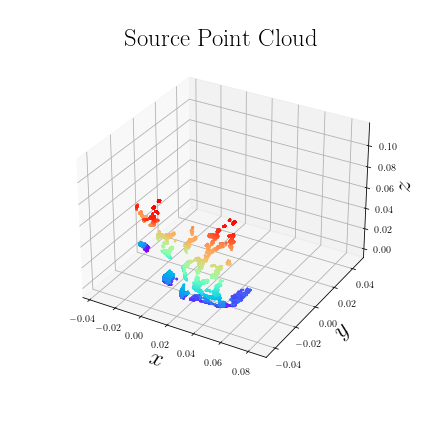
\includegraphics[width=\textwidth]{chapters/1-tactile-perception/fig/matplotlib/pc_source.png}
		\caption{The source data \mat{X} \gls{pc} generated from simulated contact points, normals are also included, but not illustrated here for the sake of simplicity.}
		\label{fig:pe-pc-source}
	\end{subfigure}
	\hfill
	\begin{subfigure}[b]{0.48\textwidth}
		\centering
		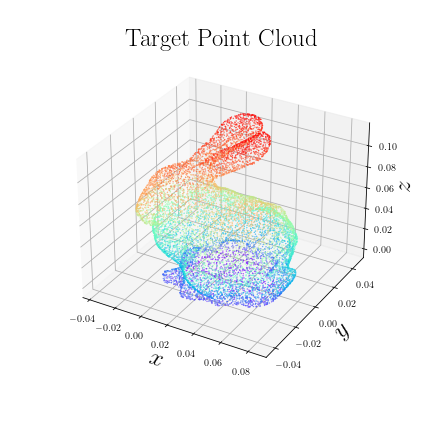
\includegraphics[width=\textwidth]{chapters/1-tactile-perception/fig/matplotlib/pc_target.png}
		\caption{The target \gls{pc} generated by sampling the model mesh with \num{10,000} points, normals are also included, but not illustrated here for the sake of simplicity.}
		\label{fig:pe-pc-target}
	\end{subfigure}
	\caption{3D plots showing source and target data.}
	\label{fig:pe-contact-position-gazebo}
\end{figure}

To determine the transformation between the two point clouds \tf[T]{\mat{X}_{src}}{\mat{Y}_{tar}}, correspondences must be found according to the \gls{corr-problem}. Due to \mvar{\mat{X}_{src}} being produced by local sensing with high-density sensor regions, a \gls{pc} feature which exploits this is desired. The one chosen is \gls{fpfh} which is a feature descriptor used in 3D point cloud analysis and registration tasks and provides a feature matrix \mvar{\mat{F}\inR{N_{pc}\times 33}}, where \mvar{N_{pc}} is the number of rows in the \gls{pc}. The feature descriptor calculates a histogram representation for each point by considering the local geometric properties of its neighboring points. It captures information about the distribution of surface normals and distances between points within a local neighborhood. Additionally, \gls{fpfh} is computationally efficient and provides robust, scale-invariant feature representations. \medskip

Once features are computed, these are used to find row matches that make up a new source and target matrices such that,
%
\begin{equation}
	\mat{X}\inR{M \times 6} \subseteq \mat{X}_{src}\inR{M_{src}\times 6} \qquad \text{and} \qquad \mat{Y}\inR{N \times 6} \subseteq \mat{Y}_{tar}\inR{N_{tar}\times 6}.
\end{equation}

These new matrices \mat{X} and \mat{Y} are the ones used from this point on as source and target matrices. \medskip

Using the correspondences found from \gls{fpfh}, the pose estimation problem can be formulated as an optimization problem for determining the optimal homogeneous transformation matrix between the two points clouds \tf[T]{\star\mat{X}}{\;\;\mat{Y}}, which for convenience is from now on referred to as \tf[T]{\star}{}, by
% \colorbox{red}{obs, what makes GNC special is the fact that it changes the \mvar{\mu} either up or down depending on GM or TLS, which gradually causes non-convexity. RCQP is used to solve for x in gnc paper}
%
\begin{equation} \label{eq:point-cloud-registration-problem}
	\tf[T]{\star}{} = \arg \min_{(\mat{R},\vec{t})\in\SE (3)} \sum^M_{i=1} d_{P_i}^{2}\left( \vec{x}_i, \mat{T} \right).
\end{equation}

Here \mvar{\tf[T]{}{}=(\tf[R]{}{}, \vec{t})\in\SE (3)} refers to the homogeneous transformation matrix \mvar{\tf[T]{}{}\inR{4\times 4}} from \mat{X} to \mat{Y}, which consists of a rotation matrix \mvar{\tf[R]{}{}\inR{3\times 3}} and a translation vector \mvar{\vec{t}\inR{3}} as members of the \gls{se} group in 3D, and \mvar{d_{P_i}(\cdot)} is the distance to the matching primitive \mvar{P_i}. The primitives of interest in this project are point-to-point and point-to-plane, due to the presence of contact normals. The distance function will differ between primitive, and thus the ones of interest are listed as
%
\begin{align}\label{eq:distance-functions}
	\min_{\vec{y}'\in P} \|\vec{x}-\vec{y}'\|^2_2 &=  \\
		& =\|\vec{x}-\vec{y}\|_2^2=\|\vec{x} - \vec{y}\|_{\mat{I}_3}^2 & \text{(point)} \\
		& = \left( \vec{n}^\T (\vec{x} - \vec{y}) \right)^2=\|\vec{x}-\vec{y}\|^2_{\vec{n}\vec{n}^\T} & \text{(plane)}
\end{align}
where \mvar{\vec{y}'\inR{3}} is the term used as a substitute for each primitive, \vec{x} is a 3D point, \mvar{\mat{I}_3\inR{3\times 3}} is the identity matrix and \mvar{\vec{n}_i} is the unit normal vector for a plane. However, these are highly sensitive to outliers and noise, and thus a robust cost function \mvar{\rho(\cdot)} is applied. Of the two presented in~\cite{graduated-non-convexity-for-robust-spatial-perception:-from-non-minimal-solvers-to-global-outlier-rejection} i.e. \gls{tls} and \gls{gm}, \gls{tls} was chosen, as it shows slightly better performance. The problem can thus be written as
%
\begin{equation}\label{eq:point-cloud-registration-problem-robust}
		\tf[T]{\star}{} = \arg \min_{(\mat{R},\vec{t})\in\SE (3)} \sum^M_{i=1} \rho\left(d_{P_i}\left( \vec{x}_i, \mat{T} \right)^{2}\right).
\end{equation}

However solving the \gls{pcr} problem globally is still a challenging endeavor, even when known correspondences are available, primarily because of the non-convex nature of the rotation constraints, where \mvar{\mat{R}\in\SE (3)}. For this reason, global approaches are applied to deal with the problem of local minima, by starting from a convex problem, and gradually increasing the non-convexity until the original problem is retrieved, this being the purpose of \gls{gnc}. However, not all solutions when found globally are of interest, as the structure of the rotation matrix places certain quadratic constraints on the solution to be valid, such as orthonormality. To solve this, a method that respects these constraints is necessary, this being the role of \gls{rcqp}. From a then estimated optimal \mvar{\mat{R}^\star}, the optimal translation \mvar{\vec{t}^\star} can be computed in a straightforward manner~\cite{convex-global-3d-registration-with-lagrangian-duality}.

\section{Method}\label{sec:2-pose-estimation-method}

% The method chosen for this chapter is twofold: first outliers are rejected using \gls{gnc} and \gls{rcqp} for determining the optimal transformation \mvar{\mat{T}^\star}. One of the common problems of \gls{pcr} is the presence of outliers, exceeding \SI{95}{\percent} is not uncommon~\cite{guaranteed-outlier-removal-for-point-cloud-registration-with-correspondences}. Outlier removal is thus necessary, which is chosen in the form \gls{gnc}. To find correspondences, a point cloud feature which utilizes the clusters of points produced by the fingertips. Thus the \gls{fpfh} descriptor is chosen. Using these features descriptors \mvar{d_{t}} are found for the target data i.e. \mat{Y} and the source data \mat{X} i.e. \mvar{d_s}. Using these matching pairs of points are found using an exhaustive search and a similarity threshold of \num{0.01}

% the distance is the normalized Euclidean distance between the matching features.

% The data is then organized in matrices \mat{X} and \mat{Y} for the source and target data, but organized such that each row corresponds 

% in the outlier-free case, we can simply solve

% \begin{equation} \label{eq:outlier-free-problem}
% 	\tf[T]{\star}{} = \arg \min_{\mat{T}\in\SE (3)} \sum^M_{i=1} r^2\left( \vec{x}_i, \tf[T]{}{} \right),
% \end{equation}

% where \mvar{\vec{x}_i} is the \mvar{i}'th sample in the data matrix \mat{X}, \mvar{\tf[T]{}{}\inR{4\times 4}} is a homogeneous transformation matrix and \mvar{\tf[T]{\star}{}\inR{4\times 4}} is the 

% quadratic cost in the least squares problem (1) with a robust cost $\rho(\cdot)$:


\subsection{Graduated Non-Convexity}\label{subs:2-pose-estimation-graduated-non-convexity}

Rather than optimizing the robust cost function \mvar{\rho(\cdot)} directly, instead a control parameter \mvar{\mu} is introduced to instead optimize
%
\begin{equation}
	\tf[T]{\star}{}=\arg \min_{(\mat{R},\vec{t})\in\SE (3)} \sum^M_{i=1} \rho_\mu \left(d_{P_i}\left(\vec{x}_i, \mat{T} \right)^{2}\right)
\end{equation}
However, since this problem cannot be solved using a non-minimal solver, the \gls{br} duality can be applied, given the necessary conditions are met. These conditions are as follows
%
\begin{align}\label{eq:br-condition-1-2-3}
	\lim_{z\rightarrow 0} \phi'(z) &= 1 & \text{condition 1} \\
	\lim_{z\rightarrow \infty}\phi'(z) &= 0 & \text{condition 2} \\
	\phi''(z) &< 0 & \text{condition 3}
\end{align}
Here \mvar{\phi(z)} is defined with respect to the robust cost function \mvar{\rho} in the following manner
%
\begin{equation}
	\phi(z) \overset{\cdot}{=} \rho(\sqrt{z}).
\end{equation}

Condition 1 indicates that as the argument \mvar{z} approaches \num{0}, the derivative of \mvar{\phi(z)} approaches \num{1}. Geometrically, it implies that near the origin, the function \mvar{\phi(z)} grows at a similar rate as the square root function itself. This behavior ensures that small values of \mvar{z} are penalized appropriately by the robust cost function \mvar{\rho(\cdot)}, allowing for robustness against outliers or deviations from the assumed distribution. \medskip

Condition 2 states that as \mvar{z} approaches \mvar{\infty}, the derivative of \mvar{\phi(z)} tends towards \num{0}. This implies that as the argument becomes larger, the function \mvar{\phi(z)} approaches a plateau or a constant value. Consequently, large values of \mvar{z} have a diminishing effect on the robust cost function, making it less sensitive to extreme observations. \medskip

Condition 3 states that the second derivative of \mvar{\phi(z)} is negative, indicating that the function \mvar{\phi(z)} is concave. This concavity is crucial as it ensures that the robust cost function \mvar{\rho(\cdot)} is monotonically increasing. In other words, as the argument \mvar{z} increases, the robust cost increases as well. This property is desirable in robust estimation problems, as it helps in downplaying the impact of outliers or influential points on the overall estimation. \medskip

All of these conditions are met by the \gls{tls}~\cite{graduated-non-convexity-for-robust-spatial-perception:-from-non-minimal-solvers-to-global-outlier-rejection}.\medskip

With these conditions fulfilled, the \gls{br} duality enables
%
\begin{equation}\label{eq:br-result}
	\arg \min_{(\mat{R},\vec{t})\in\SE (3)} \sum^M_{i=1} \rho_\mu \left(d_{P_i}\left( \vec{x}_i,\mat{T} \right)^{2}\right) = 
	\arg \min_{\substack{(\mat{R},\vec{t})\in\SE (3),\\ w_i\in [0,1]}} \sum^M_{i=1} \left[ w_i d_{P_i}\left( \vec{x}_i,\mat{T} \right)^{2} + \Phi_{\rho_\mu}(w_i)\right],
\end{equation}
where the rightmost side will be the problem of interest. In this expression \mvar{w_i\in[0,1]\forall i=1,2,\dots,M} are weights associated with each measurement \mvar{\vec{x}_i} and the outlier process function \mvar{\Phi_{\rho_\mu}(w_i)}, which computes a penalty based on the weight. The exact shape of \mvar{\Phi_{\rho_\mu}(w_i)} is determined by the chosen robust cost function. \medskip

\mvar{\Phi_{\rho_\mu}(w_i)} can simply be computed by
%
\begin{equation}
	\Phi_{\rho_\mu}(w_i) = \frac{\mu(1-w_i)}{\mu+w_i}\bar{c}^2,
\end{equation}
where \mvar{\mu} is the control parameter used to dictate to what extent the \mvar{\Phi_{\rho_\mu}(w_i)} should be convex or non-convex. For \gls{tls} \mvar{\Phi_{\rho_\mu}(w_i)} will become less convex as \mvar{\mu\rightarrow \infty}, while completely convex at \mvar{\mu=0}. This effect can be seen in~\figref{fig:tls-cost}.

\begin{figure}[!h]
	\begin{center}
		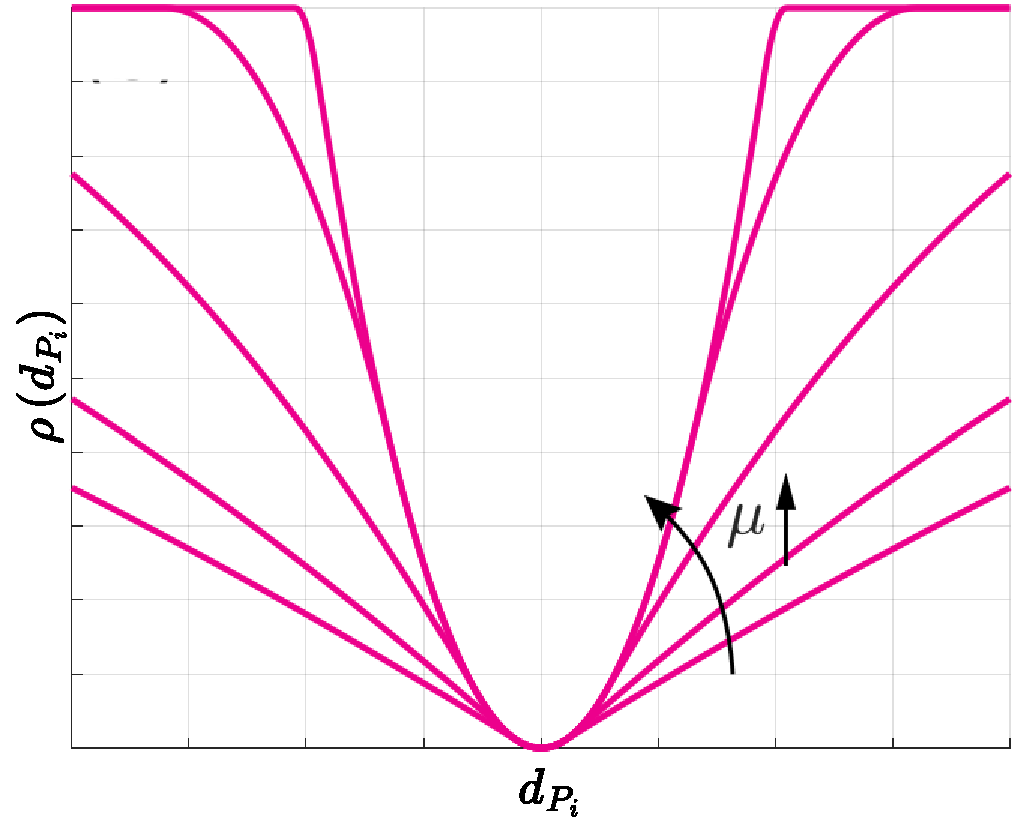
\includegraphics[width=0.3\textwidth]{chapters/2-pose-estimation/fig/tls-cost.pdf}
	\end{center}
	\caption{Cost function for the \gls{tls} with control parameter \mvar{\mu}}
	\label{fig:tls-cost}
\end{figure}
\mvar{\bar{c}^2} is a given truncation threshold, which in practice is set to the maximum error expected for the inliers. Finally, \mvar{w_i} can be computed when using \gls{tls} by
%
\begin{equation}\label{eq:tls-weights}
	w_i^{(t)} = \begin{cases}
		0 & \text{ if } \hat{r}_i^2\in\left[ \frac{\mu+1}{\mu}\bar{c}^2, +\infty \right] \\
		\frac{\bar{c}}{\hat{r}_i}\sqrt{\mu(\mu+1)} - \mu & \text{ if } \hat{r}_i^2\in\left[ \frac{\mu}{\mu+1}\bar{c}^2, \frac{\mu + 1}{\mu}\bar{c}^2 \right] \\
		1 & \text{ if } \hat{r}_i^2\in\left[ 0, \frac{\mu}{\mu + 1}\bar{c}^2 \right] \\
	\end{cases}
\end{equation}
where \mvar{\hat{r}_i^2\overset{\cdot}{=} d_{P_i}(\cdot)^2}. \eqref{eq:br-result} can now be solved through a two-step alternating optimization process. First, an outer loop is defined which increases control parameter \mvar{\mu} from \num{0} to \mvar{\infty}, until a stop criterion, dictated by the cost function, is met.~\cite{graduated-non-convexity-for-robust-spatial-perception:-from-non-minimal-solvers-to-global-outlier-rejection} found that an increase of \mvar{\mu} by a factor of \num{1.4} provided satisfactory results.
The inner loop is two-fold 1) the current estimate of \tf[T]{(t)}{} is computed by optimizing over \tf[T]{}{} with fixed weights \mvar{w_i}, also referred to as the variable update step. The variable update step can thus be written as
%
\begin{equation}\label{eq:variable-update}
	\tf[T]{(t)}{} = \arg\min_{(\mat{R},\vec{t})\in\SE (3)} \sum^N_{i=1}w_i^{(t-1)}d_{P_i}(\vec{x}_i,\mat{T}) + \underbrace{\Phi_{\rho_\mu}\left(w_i^{(t-1)}\right)}_{\text{constant}}
\end{equation}

This optimization problem is non-convex and is solved using \gls{rcqp}, which is described in~\secref{subs:2-pose-estimation-relaxed-convex-quadratic-programming}. 2) the found \tf[T]{}{} is then used to update the weights \mvar{w_i\forall i =1,2,\dots, N}, which typically can be solved in closed form, as formulated in~\eqref{eq:tls-weights}, which also is referred to as the weight update step. \medskip

When executing \gls{gnc} in practice, values are needed for \mvar{\mu_0} and \mvar{\vec{w}^{(0)}}, i.e. the parameters' initial values, along with an update rule for \mvar{\mu} and a stopping criterion. 
In this project the initial value for \mvar{\mu} is \mvar{\mu_0=2r_{\max}^2/\bar{c}^2} where \mvar{r_{\max}^2 \overset{\cdot}{=}\max_i \left(r^2(\vec{x}_i,\mat{T}^{(0)})\right)}, meaning the maximum residual after the first variable update, while \mvar{\vec{w}^{(0)}_i=1 \forall i=1,2,\dots,N}. The update rule used for \mvar{\mu} is \mvar{\mu\leftarrow 1.4\mu}, and as mentioned previously \mvar{\bar{c}^2} is set to the maximum error expected for the inliers. For \gls{tls} a fitting stop criterion is chosen to be the sum weighted squared residuals, i.e.
\begin{equation}
	\sum^N_{i=1}w_i\hat{r}_i^2.
\end{equation}
These initial values, update rules and stop criterion are based on the discoveries of~\cite{graduated-non-convexity-for-robust-spatial-perception:-from-non-minimal-solvers-to-global-outlier-rejection}. The \gls{gnc} algorithm can be seen summarized in~\algoref{alg:gnc}.

\begin{algorithm}
	\floatname{algorithm}{Algorithm}
	\algrenewcommand\algorithmicrequire{\textbf{Input: }}
	\algrenewcommand\algorithmicensure{\textbf{Output: }}
	\caption{\gls{gnc} algorithm when using \gls{tls} as \mvar{\rho(\cdot)}}
	\label{alg:gnc}
	\begin{algorithmic}[1]
		\Require matching pairs (\mat{X},\mat{Y}) with potential outliers.
		\Ensure (\mvar{\mat{X}_{in},\mat{Y}_{in}}), stats
		\State \mvar{\mu \gets 2r_{\max}^2/\bar{c}^2}
		\While {true} // outer loop
			\State $\mu\gets 1.4\mu$
			\State $\mat{R}^{(t)} \gets $ Variable Update
			\State $\vec{w}^{(t)} \gets $ Weight Update
			\If{$\sum^N_{i=1}w_i\hat{r}_i^2$ has converged}
				\State \textbf{break}
			\EndIf
		\EndWhile
		\State \textbf{return} (\mvar{\mat{X}_{in},\mat{Y}_{in}}), stats
	\end{algorithmic}
\end{algorithm}

In~\algoref{alg:gnc} the stats output generally contains information about the algorithm execution such as execution time, number of iterations, and the weights \vec{w}, while the source \mvar{\mat{X}_{in}} and target \mvar{\mat{Y}_{in}} inliers are subsets of \mat{X} and \mat{Y} with true correspondence according to \gls{gnc}. \medskip

After \gls{gnc} has converged and the inlier source \mvar{\mat{X}_{in}} and target \mvar{\mat{Y}_{in}} point matches are found, a final iteration of \gls{rcqp} is executed on the inliers for a final estimate of \tf[T]{\star}{}.

% \gls{gnc} refers to a phenomenon that arises in optimization problems where the objective function exhibits non-convexity and has multiple local optima. In contrast to traditional non-convex optimization, \gls{gnc} exploits the presence of these local optima to find better solutions progressively. \medskip

% To understand \gls{gnc}, let's start by defining some terms. In optimization, a convex function is one that has a unique global minimum. Mathematically, a function \mvar{f(\vec{x})} defined on a convex set \mat{X} is convex if for any two points \mvar{\vec{x}_1} and \mvar{\vec{x}_2} in \mat{X} and any $\lambda \in [0,1]$, the following inequality holds:
% \begin{equation}
% 	f(\lambda \vec{x}_1 + (1-\lambda)\vec{x}_2) \leq \lambda f(\vec{x}_1) + (1-\lambda)f(\vec{x}_2)
% \end{equation}

% This inequality essentially means that the function lies below the line segment connecting any two points on its graph. Convex optimization is a well-studied field with efficient algorithms for finding the global minimum.

% However, many real-world problems involve non-convex functions, which may have multiple local minima, saddle points, or other complex structures. Traditional optimization methods struggle with non-convex problems because they can get stuck in local optima, unable to find the global optimum.

% \gls{gnc} takes a different approach. Instead of trying to escape local optima, it leverages them to improve the optimization process. The idea is to gradually increase the level of non-convexity in the objective function during optimization. This process allows the algorithm to refine its solution by escaping local optima at a controlled pace.

% A common technique used in GNC is to introduce a parameter $t$ that controls the level of non-convexity. As \mvar{t} increases, the objective function becomes more non-convex. The optimization algorithm starts with a low value of $t$ where the objective function is approximately convex. It then gradually increases $t$ over time, exploring the non-convex landscape.

% The introduction of $t$ is often done by incorporating a regularization term into the objective function. The regularization term helps to maintain the properties of the convex function, ensuring that the optimization algorithm does not diverge. As $t$ increases, the regularization term becomes less significant compared to the non-convex part of the objective function, allowing the algorithm to escape local optima.

% A common form of the objective function in GNC is:

% \begin{equation}
% 	F_t(x) = f(x) + t\phi(x)
% \end{equation}

% where $f(x)$ is the original non-convex function to be optimized, $\phi(x)$ is a convex regularization term, and $t$ is the parameter controlling the non-convexity level.

% The choice of the regularization term $\phi(x)$ depends on the problem at hand and the desired behavior of the optimization algorithm. It should be designed in such a way that it encourages exploration of the non-convex landscape as $t$ increases.

% During the optimization process, as $t$ gradually increases, the algorithm starts with a nearly convex objective and finds a solution that is close to a local optimum. Then, it gradually explores the non-convex landscape by increasing the influence of the non-convex part of the objective function. This exploration helps the algorithm find better solutions that are not trapped in local optima.

% In summary, Graduated Non-Convexity is a technique used in optimization problems with non-convex objective functions. It gradually increases the level of non-convexity to explore the landscape and escape local optima. By incorporating a regularization term that maintains convexity at

% Let's consider a specific optimization problem with a non-convex objective function $f(x)$ that we want to minimize. We introduce a parameter $t$ to control the level of non-convexity.

% First, let's define the problem in a matrix and vector form. Suppose we have a vector of variables $x \in \mathbb{R}^n$ and a matrix $A \in \mathbb{R}^{m \times n}$ representing the problem's constraints. The optimization problem can be formulated as:

% \begin{align*}
% \text{minimize} & \quad f(x) \\
% \text{subject to} & \quad Ax \leq b,
% \end{align*}

% where $b \in \mathbb{R}^m$ is the vector of constraint values.

% To incorporate Graduated Non-Convexity, we introduce a convex regularization term $\phi(x)$ that helps maintain the properties of a convex function. The objective function $F_t(x)$ becomes:

% \begin{equation}
% 	F_t(x) = f(x) + t\phi(x).
% \end{equation}


% Here, $t$ controls the level of non-convexity, and as $t$ increases, the influence of the non-convex part ($t\phi(x)$) becomes more significant.

% For example, let's consider a simple case where $f(x)$ is a quadratic function and $\phi(x)$ is a convex regularization term. We can express $f(x)$ using a matrix form as:

% \begin{equation}
% 	f(x) = \frac{1}{2} x^T Q x + c^T x,
% \end{equation}

% where $Q \in \mathbb{R}^{n \times n}$ is a symmetric positive semi-definite matrix, and $c \in \mathbb{R}^n$ is a vector.
% The convex regularization term $\phi(x)$ can be written as:

% \begin{equation}
% 	\phi(x) = g(Dx),
% \end{equation}

% where $D \in \mathbb{R}^{p \times n}$ is a matrix, and $g(\cdot)$ is a convex function.

% The objective function $F_t(x)$ with GNC can be written as:

% \begin{equation}
% 	F_t(x) = \frac{1}{2} x^T Q x + c^T x + t g(Dx).
% \end{equation}

% Now, during the optimization process, we start with a small value of \mvar{t} e.g., \mvar{t = 0} where the objective function is approximately convex. We solve the optimization problem using traditional convex optimization techniques, such as quadratic programming, to find a solution \mvar{x_0} that is close to a local optimum.

% Then, we gradually increase \mvar{t} over time, which increases the non-convexity of the objective function. As \mvar{t} increases, the regularization term becomes less significant compared to the non-convex part \mvar{t g(Dx)}, allowing the algorithm to explore the non-convex landscape and potentially escape local optima.

% The specific choice of the convex regularization term \mvar{\phi(x)} and the function \mvar{g(\cdot)} depends on the problem at hand. Common choices include the \mvar{\ell_1} norm, total variation, or other convex functions that encourage certain properties or structures in the solution.

% In summary, the math behind Graduated Non-Convexity involves introducing a parameter \mvar{t} to control the level of non-convexity and incorporating a convex regularization term \mvar{\phi(x)}


% Step 1: Initialize the algorithm

% \begin{align*}
% &\text{Set } t = t_0 \text{ initial value of } t \\
% &\text{Set } x_0 \text{ as an initial feasible solution} \\
% &\text{Set iteration counter } k = 0
% \end{align*}


% Step 2: Solve the convex subproblem

% \begin{align*}
% &\text{Solve the following convex subproblem to obtain a solution } x_k: \\
% &\quad \min_{x} \frac{1}{2}x^TQx + c^Tx \\
% &\quad \text{subject to } Ax \leq b
% \end{align*}

% Step 3: Update the parameter \mvar{t}
% % \begin{align*}
% % &\text{Update } t \text{ based on a predefined schedule, e.g., } t = g(k) \text{ for some function } g(\cdot) \\
% % &\text{Increment } k \text{ by 1 (} k = k + 1\text{)}
% % \end{align*}

% Step 4: Update the objective function

% \begin{align*}
% &\text{Compute the convex regularization term: } \phi(x_k) \\
% &\text{Update the objective function with the increased non-convexity: } \\
% &\quad F_t(x) = \frac{1}{2}x^TQx + c^Tx + t\phi(x)
% \end{align*}

% Step 5: Solve the updated non-convex problem

% \begin{align*}
% &\text{Solve the following non-convex problem to obtain a new solution } x_{k+1}: \\
% &\quad \min_{x} F_t(x)
% \end{align*}

% Step 6: Check termination criteria

% \begin{align*}
% &\text{If termination criteria are satisfied, stop and return the current solution } x_{k+1} \\
% &\text{Otherwise, go to Step 3}
% \end{align*}

% In Step 2, the convex subproblem represents a traditional convex optimization problem that can be solved using various techniques such as quadratic programming or linear programming.

% In Step 4, the convex regularization term $\phi(x_k)$ can take different forms based on the problem requirements. For example, if $\phi(x_k)$ is based on the $\ell_1$ norm, it can be computed as $\phi(x_k) = \|Dx_k\|_1$ where $D$ is a matrix that determines the sparsity pattern.

% In Step 6, the termination criteria can be defined based on the problem's requirements or convergence properties, such as reaching a maximum number of iterations, achieving a desired objective value, or satisfying certain optimality conditions.

% The algorithm iteratively solves a sequence of convex subproblems and updated non-convex problems, gradually increasing the non-convexity level with the parameter \mvar{$t$}. By exploring the non-convex landscape, the algorithm aims to escape local optima and find better solutions.

% Remember that the specific implementation details of the GNC algorithm may vary depending on the problem, the chosen convex regularization term, and the optimization techniques used in solving the convex subproblems.

\subsection{Relaxed Convex Quadratic Programming} \label{subs:2-pose-estimation-relaxed-convex-quadratic-programming}

% Chapter: Tight Dual Relaxation for Non-Convex Optimization

To compute the optimal transformation matrix \tf[T]{\star}{}, the problem definition can be expressed purely in terms of \tf[R]{}{}, after which the optimal translation \mvar{\vec{t}^\star} can be computed. This simplifies the optimization problem and is therefore preferred. To do so, it will be derived from the optimization problem involving the full transformation matrix \tf[T]{}{}, formulated as
%
\begin{equation}\label{eq:linear-in-r-and-t}
	d_{P_i}^2(\vec{x}_i, \mat{T})=(\mat{T}\oplus \vec{x}_i - \vec{y}_i)^\T\mat{C}_i (\mat{T}\oplus \vec{x}_i - \vec{y}_i).
\end{equation}
Here \mvar{\mat{C}_i\inR{3\times 3}} is a symmetric matrix determined by the primitive as written in~\eqref{eq:distance-functions} and \mvar{\mat{T}\oplus \vec{x}_i} is the Euclidean transformation of \mvar{\vec{x}_i}, which is an expression linear in \tf[R]{}{} and \vec{t} i.e.
%
\begin{equation}
	\tf[T]{}{} \oplus \vec{x}_i = \mat{R}\vec{x}_i + \vec{t} = \left( \tilde{\vec{x}}^\T \otimes \mat{I}_3\right) \text{vec}(\mat{T}).
\end{equation}
Here \mvar{\tilde{\vec{x}}=\rvec{\vec{x}^\T, 1}^\T} is the homogeneous coordinate of \vec{x}, \mvar{\otimes} is the Kronecker product and \mvar{\text{vec}(\mat{T})} is the vectorization of \mat{T} i.e.
%
\begin{align}
	\text{vec}(\mat{T}) &= \rvec{\text{vec}(\mat{R})^\T, \vec{t}^\T}^\T \\
	&= \rvec{r_{11},r_{12},\dots,r_{32},r_{33},t_{1},t_{2},t_{3}}^\T \inR{12}.
\end{align}
Using this linear relationship in \mat{T},~\eqref{eq:linear-in-r-and-t} can be reformulated as 
%
\begin{equation}\label{eq:quadratic-nature}
	d_{P_i}(\vec{x}_i,\mat{T})=\tilde{\vec{\tau}}^\T \mat{N}_i^\T \mat{C}_i \mat{N}_i \tilde{\vec{\tau}}
\end{equation}
where \mvar{\vec{\tau}=\text{vec}(\mat{T})}, \mvar{\tilde{\vec{\tau}}} is the homogenized \mvar{\text{vec}(\mat{T})} i.e. \mvar{\rvec{\text{vec}(\mat{T})^\T,1}^\T}, and \mvar{\mat{N}_i=\rvec{\tilde{\vec{x}}_i^\T \otimes \mat{I}_3 | -\vec{y}_i }\inR{3\times 10}}. Due to the quadratic nature of~\eqref{eq:quadratic-nature}, it is possible to reorganize the observations and compress all the data into a single matrix \mvar{\tilde{\mat{M}}}, build from \mvar{\tilde{\mat{M}}_i = \mat{N}_i^\T \mat{C}_i \mat{N}_i\inR{13\times 13}}, meaning 
%
\begin{equation}
	f(\mat{T})=\sum^N_{i=1} d_{P_i}^2(\vec{x}_i,\mat{T})=\tilde{\vec{\tau}}^\T \left( \sum^N_{i=1} \tilde{\mat{M}}_i \right) \tilde{\vec{\tau}} = \tilde{\vec{\tau}}^\T \tilde{\mat{M}} \tilde{\vec{\tau}}.
\end{equation}
Here \mvar{f(\mat{T})} is a quadratic objective function. From this expression, it can now be seen that the size of the problem has been made independent of \mvar{N}. By then applying marginalization to the unconstrained parts of the known \mat{T} i.e. the translation \vec{t}, further compression of the problem is achieved, such that the optimal \mvar{f^\star} is written as
%
\begin{equation}\label{eq:prep-primary-problem}
	f^\star = \min_{\mat{R}\in \SE (3)} \tilde{\vec{r}}^\T \tilde{\mat{Q}} \tilde{\vec{r}} \qquad, \qquad \tilde{\vec{r}}=\rvec{\text{vec}(\mat{R})^\T, 1}^\T.
\end{equation}
Here \mvar{\tilde{\mat{Q}}} is the Schur complement of the block matrix \mvar{\tilde{\mat{M}}_{t,t}} in \mvar{\tilde{\mat{M}}}. Here the \mvar{t} subscript indicates the indexes corresponding to the translation variables and
\begin{equation}
	\mat{Q} = \tilde{\mat{M}}_{!t,!t} - \tilde{\mat{M}}_{!t,t}\tilde{\mat{M}}_{t,t}\inv \tilde{\mat{M}}_{t,!t}
\end{equation}
with \mvar{!t} being the complement of \mvar{t}.\medskip 

Although the problem is originally non-convex, it can be relaxed by applying Lagrangian relaxation to facilitate its solution. Even though a formal proof is not presented, empirical evidence from~\cite{convex-global-3d-registration-with-lagrangian-duality} demonstrates that this relaxation method consistently produces results that are close to the globally optimal solution for the marginalized problem. \medskip

Solving this non-convex optimization problem is achieved by applying Lagrangian duality to define two problems, a primary problem~\ref{eq:P} and a dual problem~\ref{eq:D}. The primary problem is an extension of~\eqref{eq:prep-primary-problem}, such that the necessary constraints for legal rotation matrices solutions are enforced, while the dual problem will be corresponding to a homogeneous version of the primal problem~\ref{eq:P}, which makes~\ref{eq:D} a Semidefinite Program (SDP), meaning the problem is convex and can be solved using off the shelf solvers. \medskip

% --------------------------------------------------------

To apply Lagrangian duality, strong duality must hold between~\ref{eq:P} and~\ref{eq:D}, meaning the solution to each of the problems are equal and their objective function values coincide. While this is not proven to hold, empirically this relaxation appears always to be tight, meaning strong duality holds, even under extreme conditions as asserted by~\cite{convex-global-3d-registration-with-lagrangian-duality}. This project will continue under the assumption that strong duality holds. \medskip

To formulate~\ref{eq:P}, the constraints of \mvar{\mat{R}\in \SE (3)} state that orthonormality and positive unit determinant must hold i.e.
%
\begin{equation}
	\mat{R}^\T\mat{R} = \mat{I}_3 \qquad \text{and} \qquad \det(\mat{R})=+1
\end{equation}

While it is appealing to formulate~\ref{eq:P} as a \gls{qcqp}, the determinant constraint is cubic and thus does not allow this formulation. In other solutions to this problem, it is not uncommon to discard the determinant constraint~\cite{lagrangian-duality-in-3d-slam:-verification-techniques-and-optimal-solutions,planar-pose-graph-optimization:-duality-optimal-solutions-and-verification} resulting in the problem only being constrained by the orthonormality constraint. This amounts to optimizing in O(3) rather than in SO(3). \medskip

Instead, by introducing additional constraints, the duality of the problem can be enhanced. Each time a new scalar constraint $c_{k+1}(\cdot)$ is incorporated into the Lagrangian, a corresponding dual variable $\lambda_{k+1}$ is introduced, and the dimension of the dual problem increases by one. This causes the new \ref{eq:D} bound \mvar{d^\star_{k+1}} to be at least as good as the previous problem's bound i.e.
%
\begin{equation}
	d^\star_{k} \le d^\star_{k+1} \le f^\star.
\end{equation}
Since this change in \ref{eq:P} causes direct changes to \ref{eq:D}, \ref{eq:D} is not intrinsic, instead it is dependant on the feasible region of \ref{eq:P}. By utilizing this property, adding more valid quadratic constraints has been shown to improve the quality of the dual relaxation~\cite[Chapter 13]{semidefinite-programming-relaxations-of-nonconvex-quadratic-optimization}. \medskip

Thus additional linearly independent quadratic constraints are added such as column and row-based orthonormality, along with additional quadratic constraints, which implicitly enforce the positive unit determinant, referred to as the rotation matrix's handedness. This constraint states that a positive unit determinant is guaranteed if the column space of \mat{R} respects the right-hand rule i.e.
%
\begin{equation}
	\mat{R}^{(1)}\times \mat{R}^{(2)} = \mat{R}^{(3)},
\end{equation}
where \mvar{\mat{R}^{(k)}} is the $k$-th column of \mat{R}. Utilizing the three possible cyclic permutations of this equation provides exactly three independent quadratic constraints, which strengthens the duality between \ref{eq:P} and \ref{eq:D}. A final constraint can be added by homogenizing~\ref{eq:P} by introducing an auxiliary variable $y$ with the constraint $y^2 = 1$. The primary problem~\ref*{eq:P} can thus be expressed as
%
\begin{align*}
	&\min_{\mat{R}} \tilde{\vec{r}}^\T \tilde{\mat{Q}} \tilde{\vec{r}}  \quad , \quad \tilde{\vec{r}}=\rvec{\text{vec}(\mat{R})^\T, y}^\T, \\
	& \text{s.t. }         \\ 
	&\qquad \qquad \mat{R}^\T\mat{R} = y^2\mat{I}_3, \tag{$\mathcal{P}$} \label{eq:P}\\
	&\qquad \qquad \mat{R}\mat{R}^\T = y^2 \mat{I}_3, \\
	&\qquad \qquad \mat{R}^{(i)}\times \mat{R}^{(j)}=y \mat{R}^{(k)} \quad , \quad i,j,k = \text{cyclic}(1,2,3), \\
	&\qquad \qquad y^2 = 1.
\end{align*}

To derive the dual problem~\ref{eq:D}, the \gls{qcqp} nature of~\ref{eq:P} is utilized to express its Lagrangian as
%
\begin{equation}\label{eq:lagrangian-p}
	\mathcal{L}(\tilde{\vec{r}}, \tilde{\vec{\lambda}}) = \gamma + \tilde{\vec{r}}^\T  \tilde{\mat{Z}}  \tilde{\vec{r}}.
\end{equation}
Here \mvar{\tilde{\vec{\lambda}}=\rvec{\vec{\lambda}^\T, \gamma}^\T\inR{22}} is the dual vector, where \num{22} is the number of constraints in~\ref{eq:P}, \mvar{\tilde{\mat{Z}}=\tilde{\mat{Q}} + \tilde{\mat{P}}(\tilde{\vec{\lambda}})} is a penalization matrix of the sum of \mvar{\tilde{\mat{Q}}}, which contains all the data from~\ref{eq:P}, and \mvar{\tilde{\mat{P}}(\tilde{\vec{\lambda}})} which is the accumulation of all the penalization terms corresponding to different constraint types. \mvar{\tilde{\mat{P}}(\tilde{\vec{\lambda}})} can be computed as
%
\begin{equation}\label{eq:penalty-matrix}
	\tilde{\mat{P}}(\tilde{\vec{\lambda}}) = \tilde{\mat{P}}_r(\mat{\Lambda}_r) + \tilde{\mat{P}}_c(\mat{\Lambda}_c) + \tilde{\mat{P}}_d(\{ \vec{\lambda}_{d_{ijk}} \}) + \tilde{\mat{P}}_h(\gamma),
\end{equation}
which by definition is a linear function of the dual variables, where the structural pattern of the involved matrices can be found in~\cite{convex-global-3d-registration-with-lagrangian-duality}. Using this formulation of the Lagrangian, its relaxation can be solved in closed form as 
\begin{align}
	d(\tilde{\vec{\lambda}})&=\min_{\tilde{\vec{r}}}\mathcal{L}(\tilde{\vec{r}},\tilde{\vec{\lambda}})=\min_{\tilde{\vec{r}}} \gamma + \tilde{\vec{r}}^\T \tilde{\vec{Z}} \tilde{\vec{r}} \\
	&= \begin{cases}
		\gamma & \text{ if } \tilde{\mat{Z}} \succeq \vec{0}, \\
		-\infty & \text{ otherwise }.
	\end{cases}
\end{align}
In cases where \mvar{\tilde{\mat{Z}}} is not \gls{psd} no lower bound exists for this problem, and thus no optimal solution can be found. But by restricting all \mvar{\tilde{\vec{\lambda}}}, to the solutions of \mvar{d(\tilde{\vec{\lambda}})} which satisfy \mvar{\tilde{\mat{Z}} \succeq \vec{0}}, the dual problem \ref{eq:D} to the homogeneous primal problem \ref{eq:P} is a Semidefinite Program on the form 
%
\begin{align*}
	& d^\star = \max_{\tilde{\vec{\lambda}}} \gamma, \\
	& \text{s.t. }         \tag{$\mathcal{D}$} \label{eq:D}\\ 
	&\qquad \qquad \tilde{\mat{Z}}(\tilde{\vec{\lambda}})=\tilde{\mat{Q}} + \tilde{\mat{P}}(\tilde{\vec{\lambda}}) \succeq 0. 
\end{align*}
Which is a semidefinite program i.e. a convex problem that can be solved by out-of-the-box solvers. \medskip

From the now defined primal problem~\ref{eq:P} and dual problem~\ref{eq:D}, and under the assumption that strong duality holds \mvar{f^\star = d^\star}, which implies by duality theory that \mvar{\tilde{\vec{r}}^\star} must be a minimizer of the Lagrangian~\ref{eq:lagrangian-p} evaluated at \mvar{\tilde{\vec{\lambda}}^\star}, such that
%
\begin{equation}
	\vec{r}^\star = \arg\min_{\vec{r}} \mathcal{L}(\vec{r},\vec{\lambda}^\star) \quad \Rightarrow \quad \left( \tilde{\vec{r}}^\star \right)^\T \tilde{\mat{Z}}^\star \tilde{\vec{r}}^\star = 0.
\end{equation}
Assuming \mvar{\tilde{\mat{Z}}^\star} is \gls{psd} i.e. \mvar{\tilde{\mat{Z}}^\star \succeq 0}, then the optimal solution \mvar{\tilde{\vec{r}}^\star} must lie in the nullspace of \mvar{\tilde{\mat{Z}}^\star} i.e. \mvar{\tilde{\vec{r}}^\star \in \text{null}\left( \tilde{\mat{Z}}^\star \right)}. If this was not the case, either \mvar{\text{null}\left( \tilde{\mat{Z}}^\star \right) = \emptyset} or \mvar{\tilde{\vec{r}}^\star \notin \text{null}\left( \tilde{\mat{Z}}^\star \right)}, as a direct consequence of \mvar{\tilde{\mat{Z}}^\star} being \gls{psd}. \medskip

From this the nullspace basis \mat{V} of \mvar{ \tilde{\mat{Z}}^\star } i.e. \mvar{\mat{V}=\text{null}\left( \tilde{\mat{Z}}^\star \right)} can be computed using QR decomposition. If it here is the case that \mvar{\text{rank}(\mat{V})=1} then the optimal solution \mvar{\vec{r}^\star} is found as the dehomogenized nullspace basis of \mvar{\tilde{\mat{Z}}}, due to~\ref{eq:P} being homogenous. \medskip
% By simply dehomogenizing \mvar{\tilde{\vec{r}}^\star}, the optimal rotation \mvar{\vec{r}^\star} is found. \medskip

Verifying the legitimacy of this solution is simply done by evaluating the nullspace determinant to be unit, and the difference between the optimal value of~\ref{eq:P} and~\ref{eq:D} being \num{0} i.e.
%
\begin{equation}
	\text{rank} \left(\text{null}( \tilde{\mat{Z}}^\star )\right) = 1 \qquad \text{ and } \qquad  d^\star - f^\star(\mat{R}^\star) = 0
\end{equation}
where \mvar{\mat{R}^\star = \text{reshape}(\vec{r}^\star)}. \medskip

The algorithm for computing the optimal \tf[R]{\star}{} can be seen summarized in~\algoref{alg:rcqp}. To compute the full optimal transformation matrix \tf[T]{\star}{}, this result is used in~\algoref{alg:t-star}, and thus the optimal homogeneous transformation matrix has been estimated using \gls{rcqp}.
% Using the optimal \tf[R]{\star}{} the optimal translation can be found using~\algoref{alg:t-star}.
% To summarize, the \gls{rcqp} algorithm can be seen in~\algoref{alg:rcqp}.

\begin{algorithm}
	\floatname{algorithm}{Algorithm}
	\algrenewcommand\algorithmicrequire{\textbf{Input: }}
	\algrenewcommand\algorithmicensure{\textbf{Output: }}
	\caption{\gls{rcqp} algorithm for determining \tf[R]{\star}{} from \mvar{\tilde{\vec{r}}^\T \tilde{\mat{Q}} \tilde{\vec{r}}}}
	\label{alg:rcqp}
	\begin{algorithmic}[1]
		\Require Marginalized quadratic form of the primary problem, \ref{eq:P} i.e. \mvar{\tilde{\vec{r}}^\T \tilde{\mat{Q}} \tilde{\vec{r}}}
		\Ensure Globally optimal \tf[R]{\star}{}, if strong duality holds
		\State \mvar{ \tilde{\mat{Z}} ( \tilde{\vec{\lambda}})  \gets } build\mvar{\left(\tilde{\mat{Q}} + \tilde{\mat{P}}(\tilde{\vec{\lambda}})\right)} based on~\ref{eq:penalty-matrix}

		\State \mvar{(\tilde{\vec{\lambda}}^\star, \tilde{\mat{Z}}^\star) \gets} \texttt{cvx}(\ref{eq:D}\mvar{(\tilde{\vec{\lambda}}, \tilde{\mat{Z}})}) i.e. solve the Semidefinite Program using optimization tools such as \texttt{cvx} 

		\State \mvar{\mat{V} \gets \text{null}(\tilde{\mat{Z}}^\star)}, from methods such as QR decomposition.

		\State \texttt{ASSERT} (rank\mvar{(\mat{V} ) == 1}), ensure the nullspace rank is unit
		\State \texttt{ASSERT} \mvar{\left( \left(\tilde{\vec{r}}^\star\right)^\T \tilde{\mat{Q}} \tilde{\vec{r}}^\star - d^\star < \epsilon \right)}  , where \mvar{\epsilon} is some threshold close to \num{0}, to ensure strong duality
		
		\State \mvar{\vec{r}^\star \gets \tilde{\vec{r}}^\star}, dehomogenize \mvar{\tilde{\vec{r}}^\star}

		\State \mvar{\tf[R]{\star}{} \gets} reshape(\mvar{\vec{r}^\star}), reshape \mvar{\vec{r}^\star\inR{9}} to \mvar{\mat{R}^\star\inR{3 \times 3}}
		\State \textbf{return} \tf[R]{\star}{}, return the globally optimal rotation
	\end{algorithmic}
\end{algorithm}

\begin{algorithm}
	\floatname{algorithm}{Algorithm}
	\algrenewcommand\algorithmicrequire{\textbf{Input: }}
	\algrenewcommand\algorithmicensure{\textbf{Output: }}
	\caption{Algorithm for determining \tf[T]{\star}{} from \mvar{\tilde{\vec{r}}^\T \tilde{\mat{Q}} \tilde{\vec{r}}}}
	\label{alg:t-star}
	\begin{algorithmic}[1]
		\Require matching paris from (\mvar{\mat{X},\mat{Y}})
		\Ensure Globally optimal \tf[T]{\star}{}
		\State initialize \mvar{\tilde{\mat{M}} \gets } zeros(\num{13})
		\For{ \mvar{(\vec{x}_i, P_i) \in \{ \vec{x}_i \leftrightarrow P_i \}^m_{i=1} } }
			\State \mvar{\tilde{\mat{M}}_i \leftarrow} buildTerm(\mvar{\vec{x}_i,P_i}) here build term depends on the primitive.
			\State \mvar{\tilde{\mat{M}} \gets \tilde{\mat{M}} + \tilde{\mat{M}}_i}
		\EndFor
		\State marginalize \mvar{\tilde{\mat{Q}} = \tilde{\mat{M}} / \tilde{\mat{M}}_{\vec{t},\vec{t}} } using Schur complement.
		\State compute \tf[R]{\star}{} from~\algoref{alg:rcqp}
		\State \mvar{\vec{t}^\star \gets -\tilde{\mat{M}}_{\vec{t},\vec{t}}^{-1} \tilde{\mat{M}}_{\vec{t}, !\vec{t}} \tilde{\vec{r}} } where \mvar{ \tilde{\vec{r}} = \rvec{\text{vec}(\mat{R})^\T 1}^\T}
		\State \textbf{return} \tf[T]{\star}{}(\tf[R]{\star}{},\mvar{\vec{t}^\star})
	\end{algorithmic}
\end{algorithm}

\newpage

\section{Experimental Setup}\label{sec:2-pose-estimation-experimental-setup}

To Test the performance of the algorithms presented in~\secref{sec:2-pose-estimation-method} two setups are needed, one for synthetic source data and one for sampled source data. \medskip

The synthetic source and target data are generated by sampling the Stanford bunny mesh uniformly with \num{1000} data points and corresponding normals. This will ensure the index \mvar{i} of each \gls{pc} will be true correspondences even if transformed. Once sampled, the synthetic source data transformed using
%
\begin{equation}
	\tf[T]{\text{Target}}{\text{Source}} = 
	\begin{bmatrix}
		\tf[R]{}{z}(\pi/4) & \vec{t}_x(1) \\
		\vec{0}_{1\times 3} & 1
	\end{bmatrix}\inR{4\times 4}.
\end{equation} 
Here \mvar{\mat{R}_z(\pi/4)\inR{3\times 3}} is the rotation matrix for a rotation of \mvar{\pi/4=45\deg} about the $z$-axis, \mvar{\vec{t}_x(1)\inR{3}} is a translation along the $x$-axis of \num{1} and \mvar{\vec{0}_{1\times 3}=\rvec{0,0,0}}. The target and synthetic source data can be seen in \figref{fig:synthetic-target-data} and~\figref{fig:synthetic-source-data} respectively. \medskip

On these points clouds \gls{gnc}+\gls{rcqp} are applied over \num{20} experiments with varying outlier percentages \mvar{\alpha=\rvec{10\%,20\%,\dots,90\%}}. \medskip

% the target data sampled from the \gls{cad} model of the object of interest i.e. the Stanford bunny. The mesh is sampled uniformly with \num{1000} data points and with corresponding normals making up the target data, while the source data is made from a homogeneous transformation matrix applied to a copy of the target data. 
% This will ensure the index \mvar{i} of each point in each point cloud will be true correspondences even when transformation. The homogeneous transformation matrix chosen is
% \begin{equation}
% 	\tf[T]{\text{Target}}{\text{Source}} = 
% 	\begin{bmatrix}
% 		\tf[R]{}{z}(\pi/4) & \vec{t}_x(1) \\
% 		\vec{0}_{1\times 3} & 1
% 	\end{bmatrix}\inR{4\times 4}
% \end{equation} 
% where \mvar{\mat{R}_z(\pi/4)\inR{3\times 3}} is the rotation matrix for a rotation of \mvar{\pi/4=45\deg} about the $z$-axis, \mvar{\vec{t}_x(1)\inR{3}} is a translation along the $x$-axis of \num{1} and \mvar{\vec{0}_{1\times 3}=\rvec{0,0,0}}. The target and synthetic source data can be seen in \figref{fig:synthetic-target-data} and~\figref{fig:synthetic-source-data} respectively.

\begin{figure}[!h]
	\centering
	\begin{subfigure}[b]{0.48\textwidth}
		\centering
		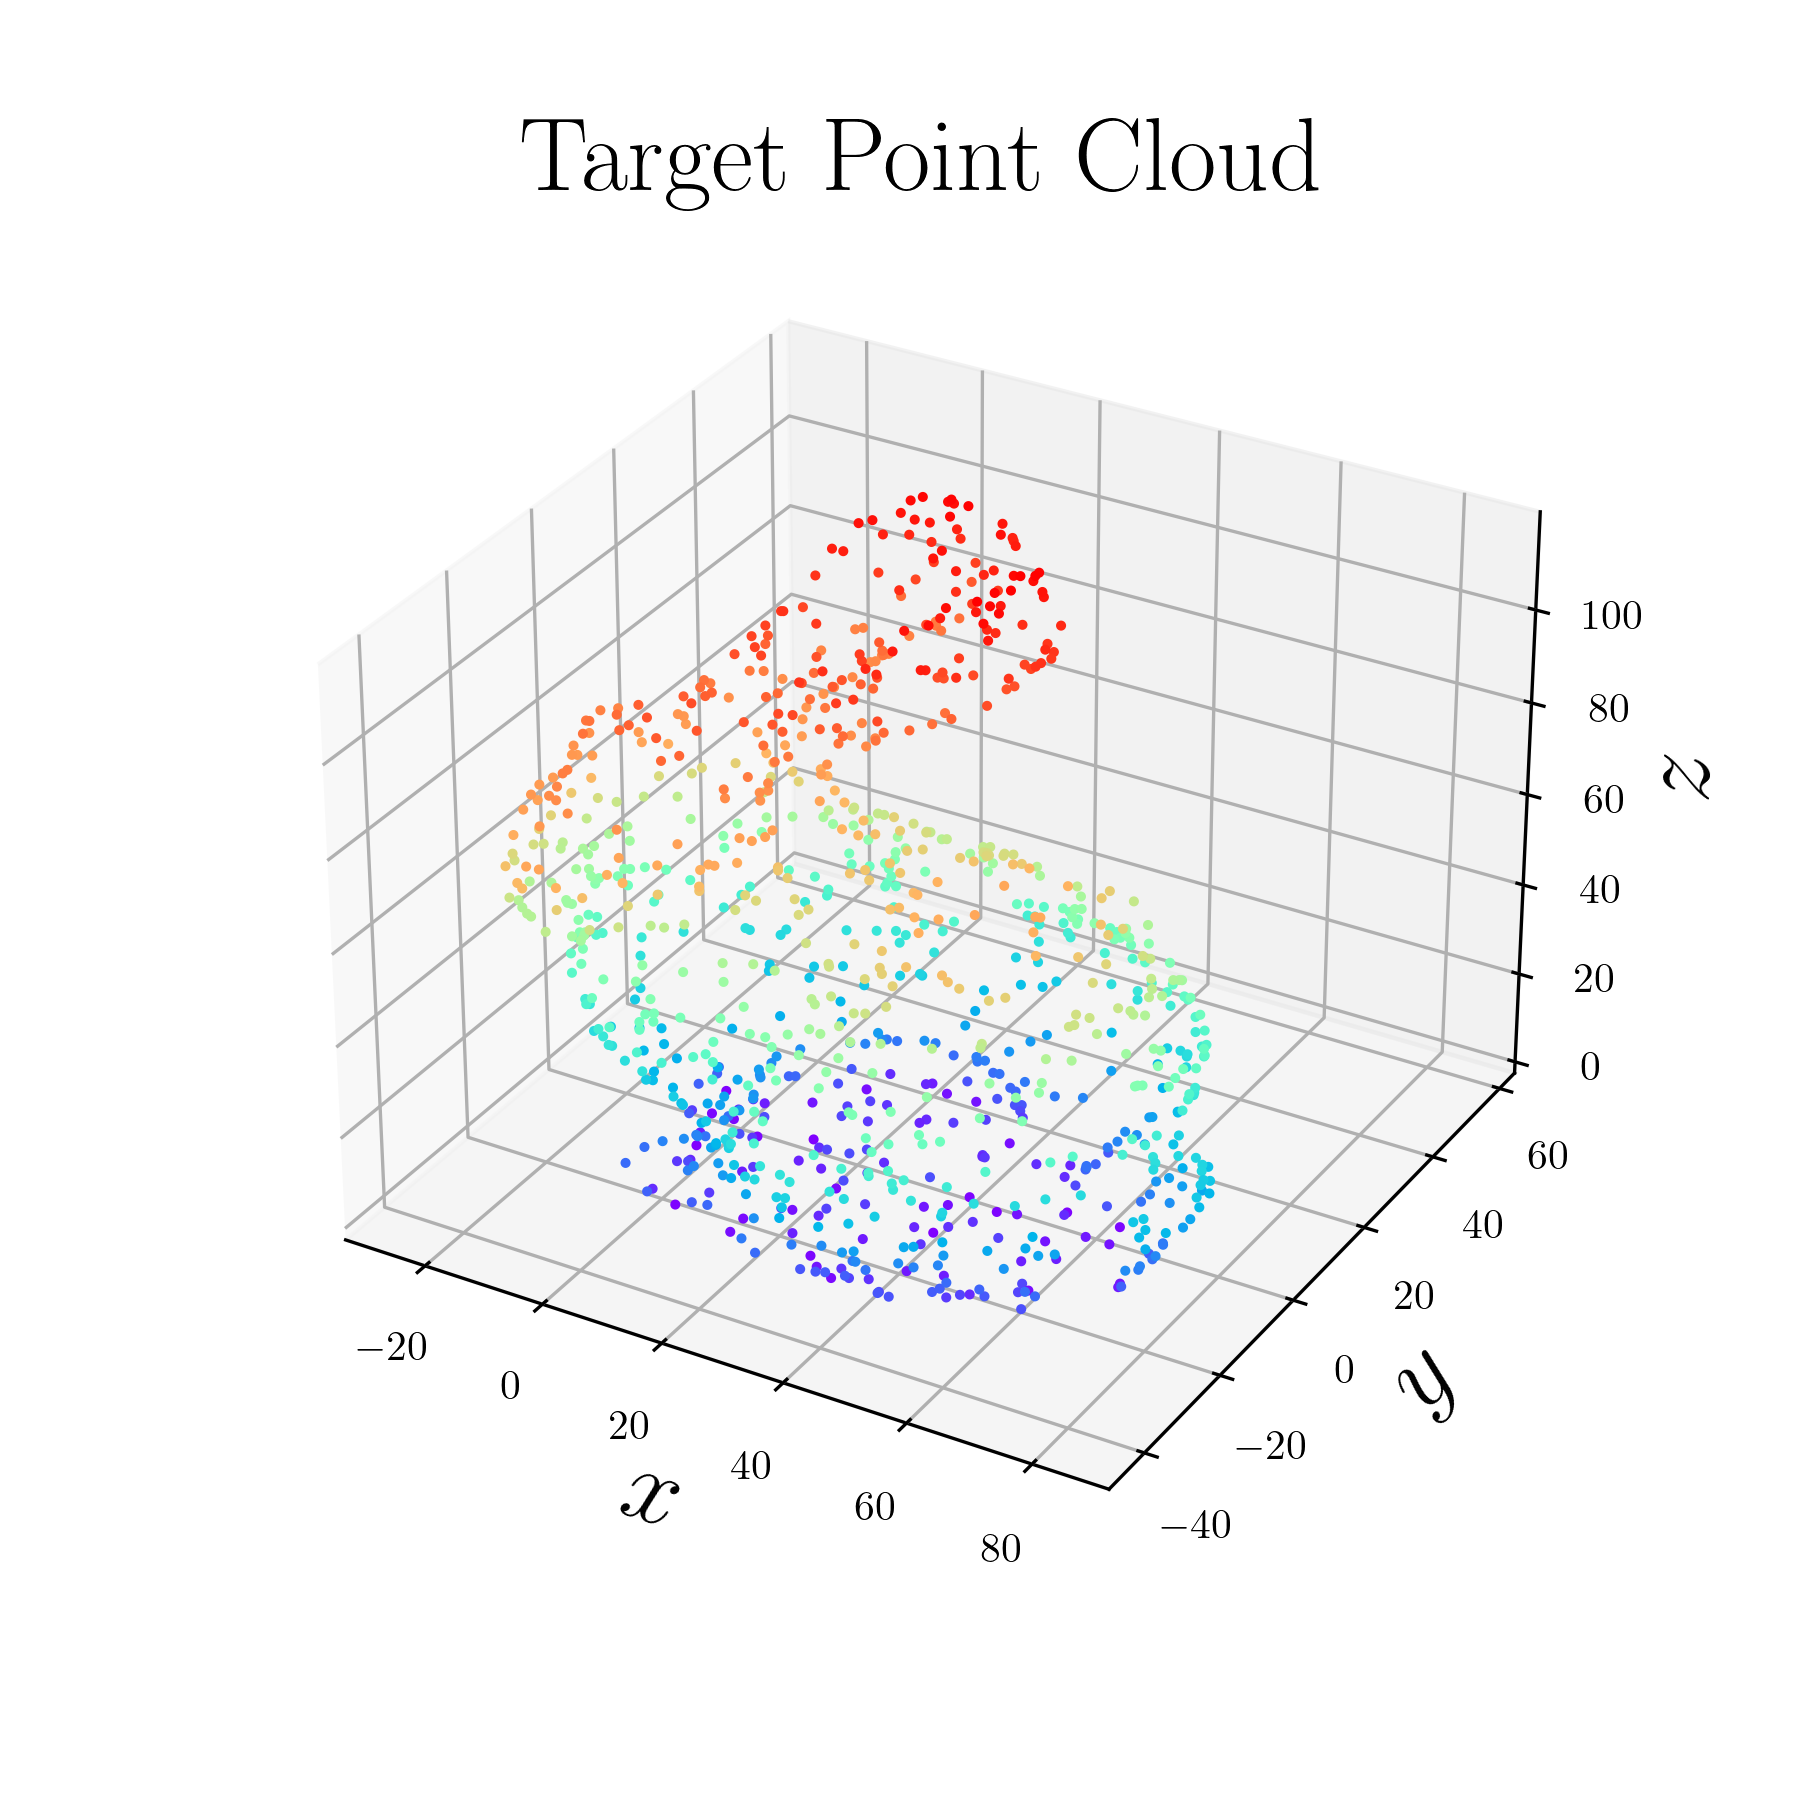
\includegraphics[width=\textwidth]{chapters/2-pose-estimation/fig/synthetic_pc_target.png}
		\caption{The target \gls{pc} generated from sampling \num{1000} points from the \gls{cad} model.}
		\label{fig:synthetic-source-data}
	\end{subfigure}
	\hfill
	\begin{subfigure}[b]{0.48\textwidth}
		\centering
		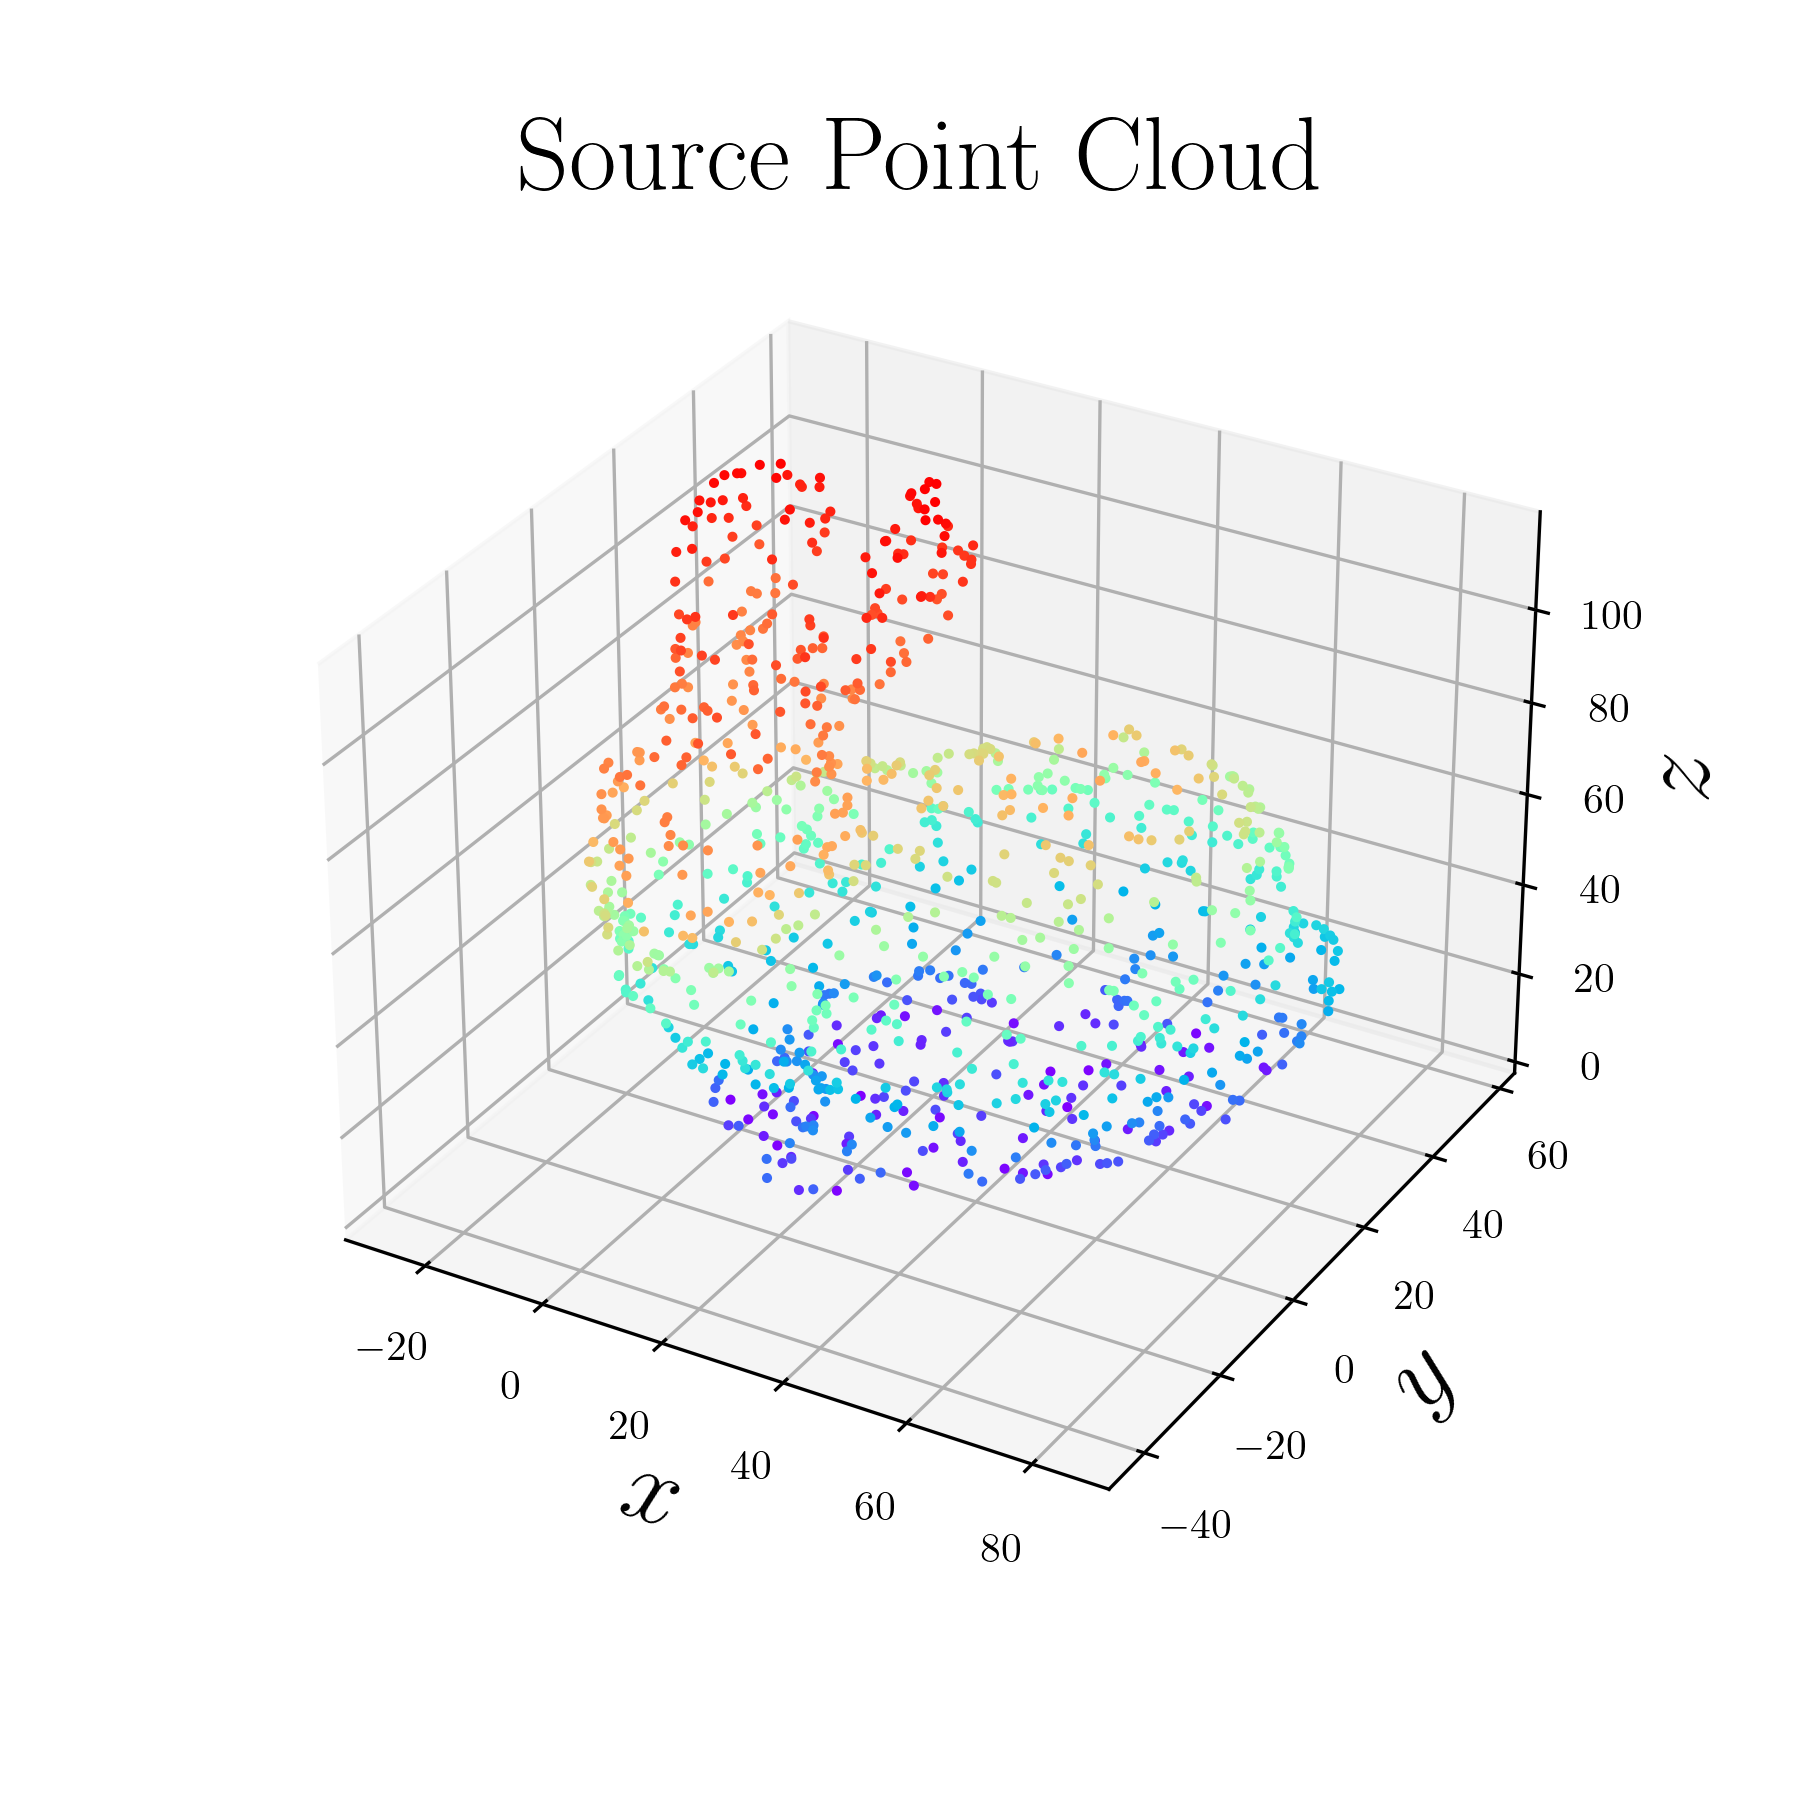
\includegraphics[width=\textwidth]{chapters/2-pose-estimation/fig/synthetic_pc_source.png}
		\caption{The synthetic source data based on the target data, but transformed \mvar{\tf[T]{\text{Target}}{\text{Source}}}.}
		\label{fig:synthetic-target-data}
	\end{subfigure}
	\caption{3D plots showing the synthetic source data and target data.}
	\label{fig:synthetic-source-and-target-data}
\end{figure}

% On these points clouds \gls{gnc}+\gls{rcqp} are applied over \num{20} experiments with varying outlier percentages \mvar{\alpha=\rvec{10\%,20\%,\dots,90\%}}. \medskip

The setup for the sampled source data as shown in~\figref{fig:pe-pc-source}, additionally includes the solving of the \gls{corr-problem} by finding feature correspondences between the sampled source \gls{pc} and target \gls{pc}. The target \gls{pc} is the same as the one generated for the synthetic source data setup. \medskip 

Due to self-collisions during the sampling process, a statistical outlier filter was applied with the number of neighbors \mvar{n_{nb}} being \num{1,000} and the standard deviation ratio \mvar{\sigma} being \num{0.5} to eliminate these outliers.\medskip

Using \gls{fpfh} it was unfortunately found that the source data did not contain enough information to find a satisfactory number of feature matches with the target data for \gls{gnc}+\gls{rcqp} to function. This was found by sampling target data with a varying number of data points uniformly distributed while computing the number of feature matches with the sampled source data. These results can be seen in~\figref{fig:number-of-feature-matches-with-different-numbers-of-target-data-points}, where the number of target data points sampled are \mvar{\gamma = \rvec{100,200,\dots,900,1000,2000,\dots,50000}} and the largest number of feature matches show to be two, which is far from sufficient. Filtering the sampled source data did not increase the number of feature matches as shown in the~\figref{fig:number-of-feature-matches-with-different-numbers-of-target-data-points}. Greater target data \gls{pc}s were attempted but were not possible due to lack of computer memory.

\begin{figure}[!h]
	\begin{center}
		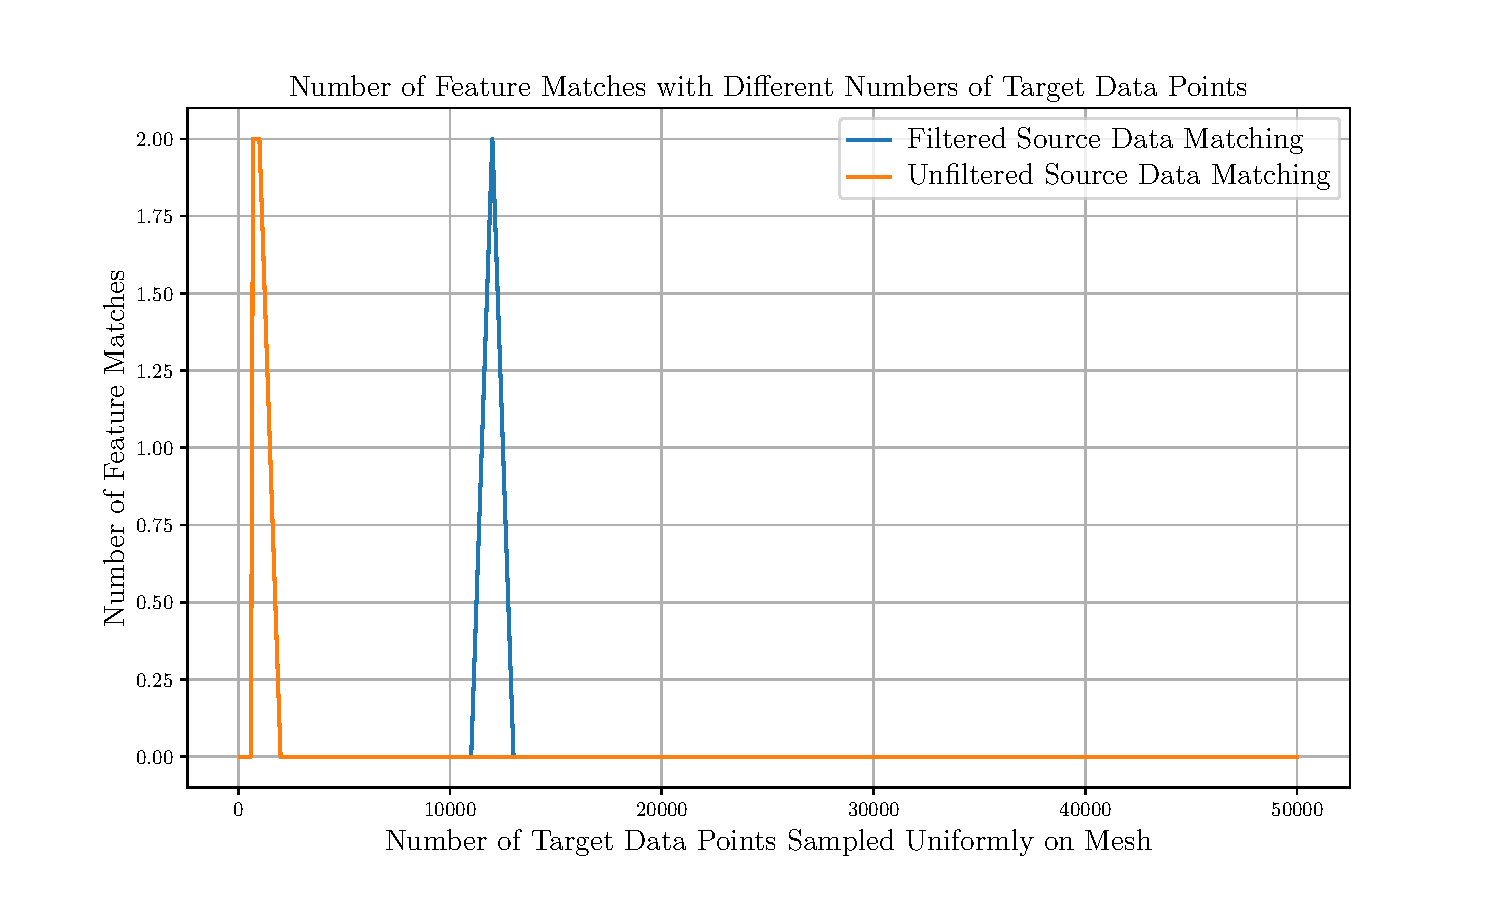
\includegraphics[width=0.8\textwidth]{chapters/2-pose-estimation/fig/number-of-feature-matches-with-different-numbers-of-target-data-points.pdf}
	\end{center}
	\caption{Number of feature matches between target data containing \mvar{\gamma} data points and the sampled source data, both filtered and unfiltered.}
	\label{fig:number-of-feature-matches-with-different-numbers-of-target-data-points}
\end{figure}
% Using these two, heatmaps were produced, where~\figref{fig:pe-feature-filtered-pc} shows the heatmap for the filtered source data while~\figref{fig:pe-feature-unfiltered-pc} shows the heatmap for the unfiltered source data. \medskip
% \begin{figure}[!h]
% 	\centering
% 	\begin{subfigure}[b]{0.48\textwidth}
% 		\centering
% 		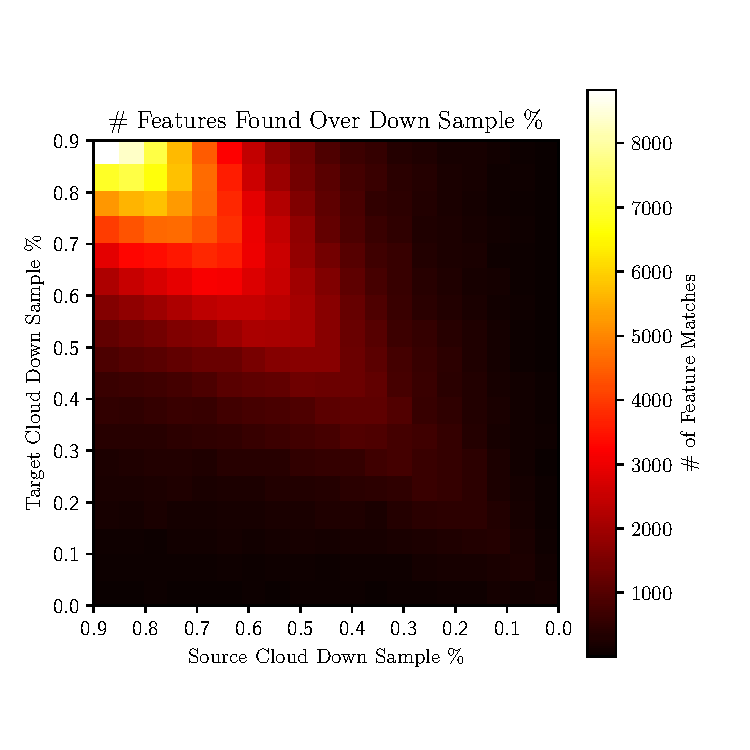
\includegraphics[width=\textwidth]{chapters/2-pose-estimation/fig/M.pdf}
% 		\caption{The source \gls{pc} generated from simulated contact points.\newline}
% 		\label{fig:pe-feature-filtered-pc}
% 	\end{subfigure}
% 	% \hfill
% 	\begin{subfigure}[b]{0.48\textwidth}
% 		\centering
% 		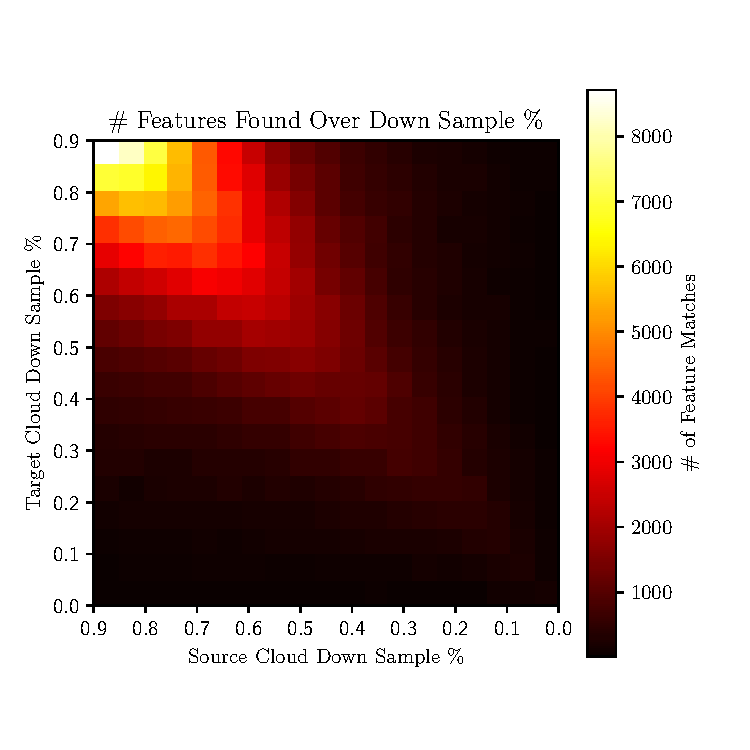
\includegraphics[width=\textwidth]{chapters/2-pose-estimation/fig/M_unfiltered.pdf}
% 		\caption{The target \gls{pc} generated by sampling the model mesh with \num{10,000} points.}
% 		\label{fig:pe-feature-unfiltered-pc}
% 	\end{subfigure}
% 	\caption{3D plots showing the sampled source and target \gls{pc}s along with a plot showing both of them overlaid.}
% 	\label{fig:pe-filture-and-unfiltered-pc}
% \end{figure}
% Here the greatest number of feature matches for the filtered source data was \num{11,450}, while \num{11,178} for the unfiltered. Since down-sampling the \gls{pc}s simply reduced the number of matches, the sample \gls{pc} used as source data is the filtered non-down sampled data i.e. the data shown in~\figref{fig:pe-pc-source}.
\section{Results}\label{sec:2-pose-estimation-results}

Using the synthetic source data the results presented in this section were found.

\subsection{Pose Estimation Performance Data}

The number of iterations for each outlier percentage can be seen as boxplots in~\figref{fig:GNC-TLS-iterations-e},~\figref{fig:GNC-TLS-time-e} shows boxplots of the execution times for each outlier percentage,~\figref{fig:GNC-TLS-theta-e} shows boxplots of the estimated orientation error as the angle \mvar{\theta_e} being the angle in \gls{eaa} format. Finally,~\figref{fig:GNC-TLS-t-e} shows boxplots of the translational error.
% \begin{figure}[!h]
% 	\centering
% 	\begin{subfigure}[b]{0.48\textwidth}
% 		\centering
% 		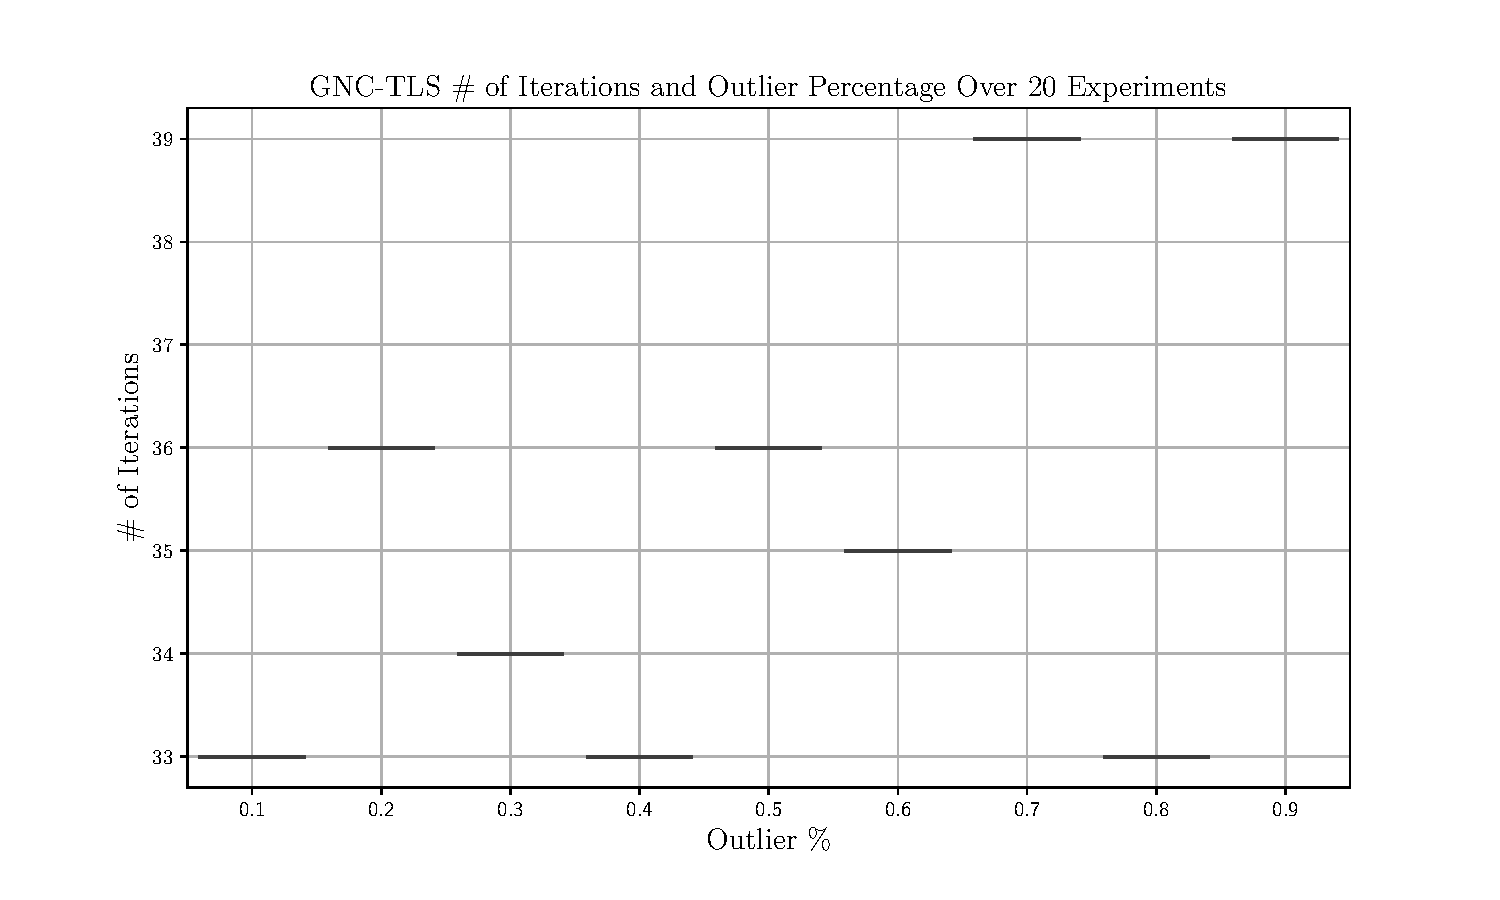
\includegraphics[width=\textwidth]{chapters/2-pose-estimation/fig/GNC-TLS-iterations-e.pdf}
% 		\caption{The source \gls{pc} generated from simulated contact points.\newline}
% 		\label{fig:pe-feature-filtered-pc2}
% 	\end{subfigure}
% 	% \hfill
% 	\begin{subfigure}[b]{0.48\textwidth}
% 		\centering
% 		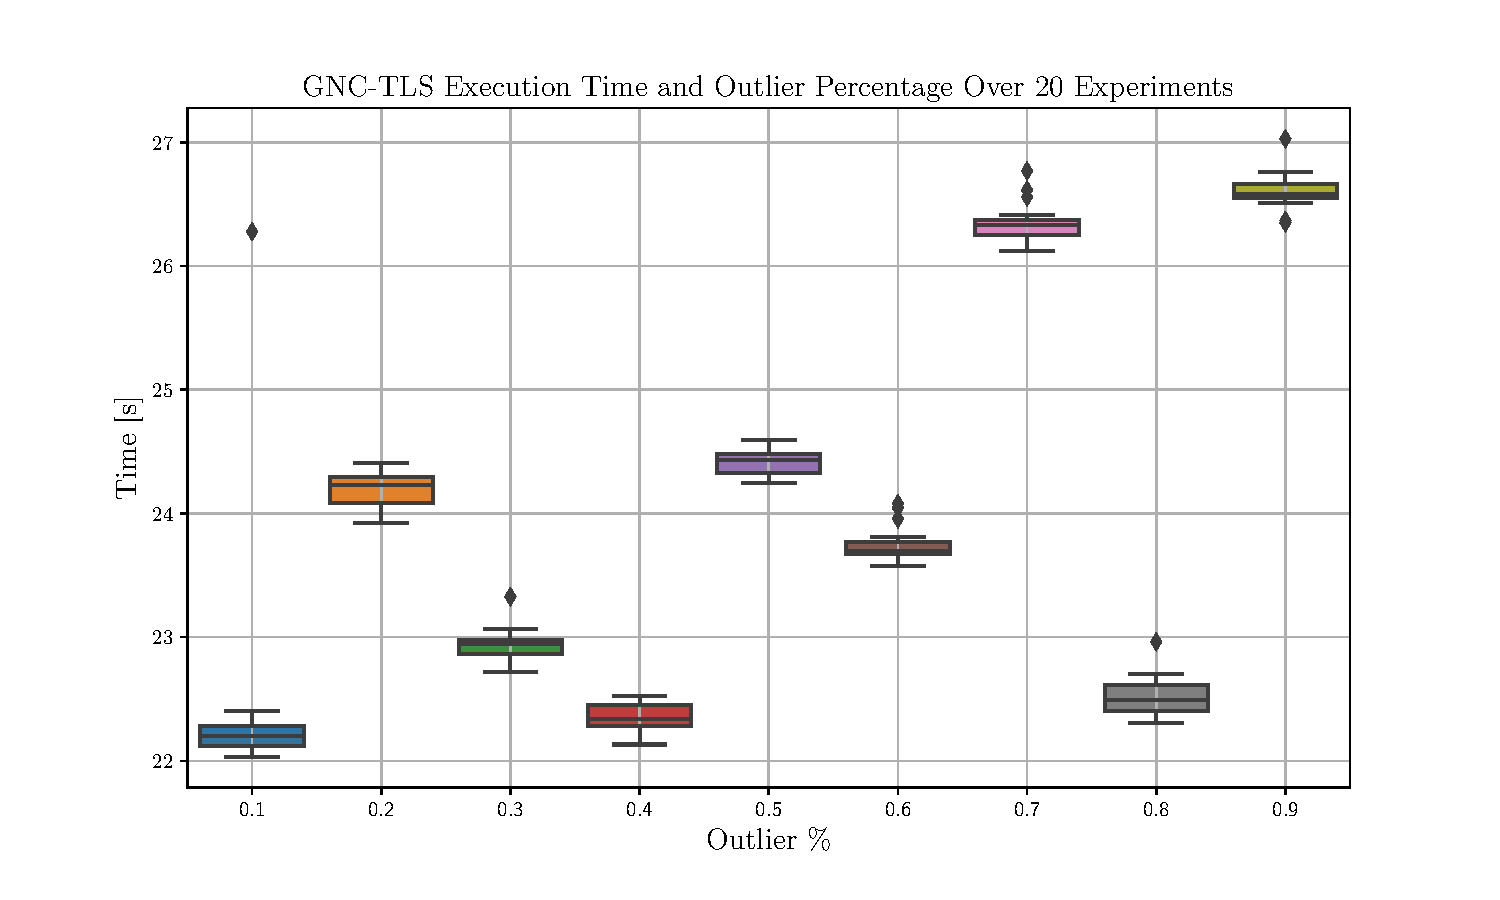
\includegraphics[width=\textwidth]{chapters/2-pose-estimation/fig/GNC-TLS-time-e.pdf}
% 		\caption{The target \gls{pc} generated by sampling the model mesh with \num{10,000} points.}
% 		\label{fig:pe-feature-unfiltered-pc2}
% 	\end{subfigure}
% 	\caption{3D plots showing the sampled source and target \gls{pc}s along with a plot showing both of them overlaid.}
% 	\label{fig:pe-filture-and-unfiltered-pc2}
% \end{figure}
\begin{figure}[!h]
	\begin{center}
		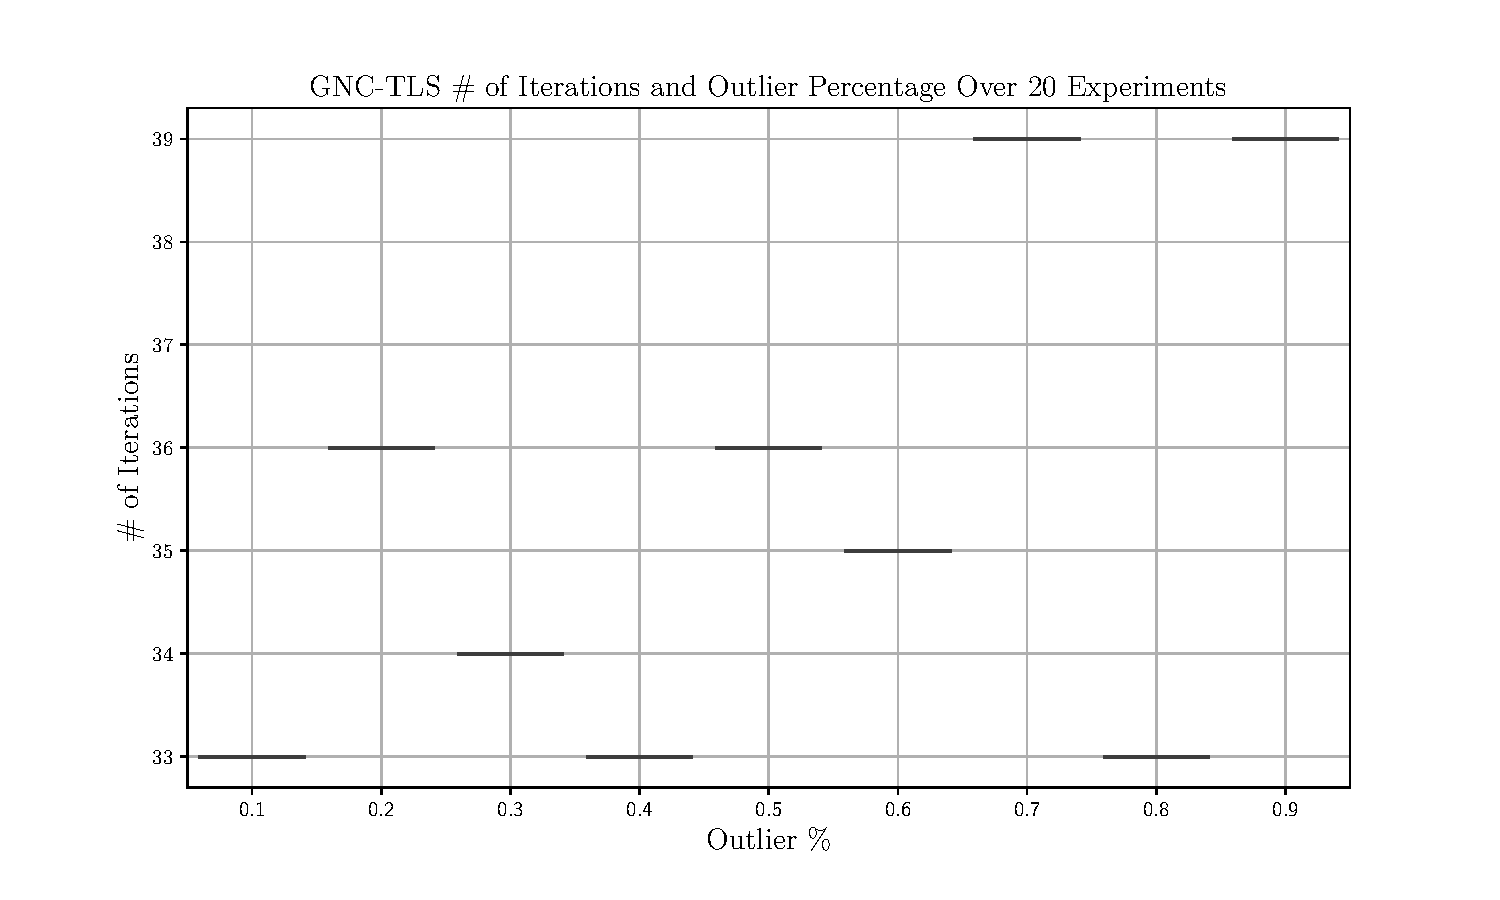
\includegraphics[width=\textwidth]{chapters/2-pose-estimation/fig/GNC-TLS-iterations-e.pdf}
	\end{center}
	\caption{Boxplots showing the number of \gls{gnc} outer loop iterations for each outlier percentage from \SI{10}{\percent} to \SI{90}{\percent} in steps of \SI{10}{\percent}, over \num{20} experiments. }
	\label{fig:GNC-TLS-iterations-e}
\end{figure}

\begin{figure}[!h]
	\begin{center}
		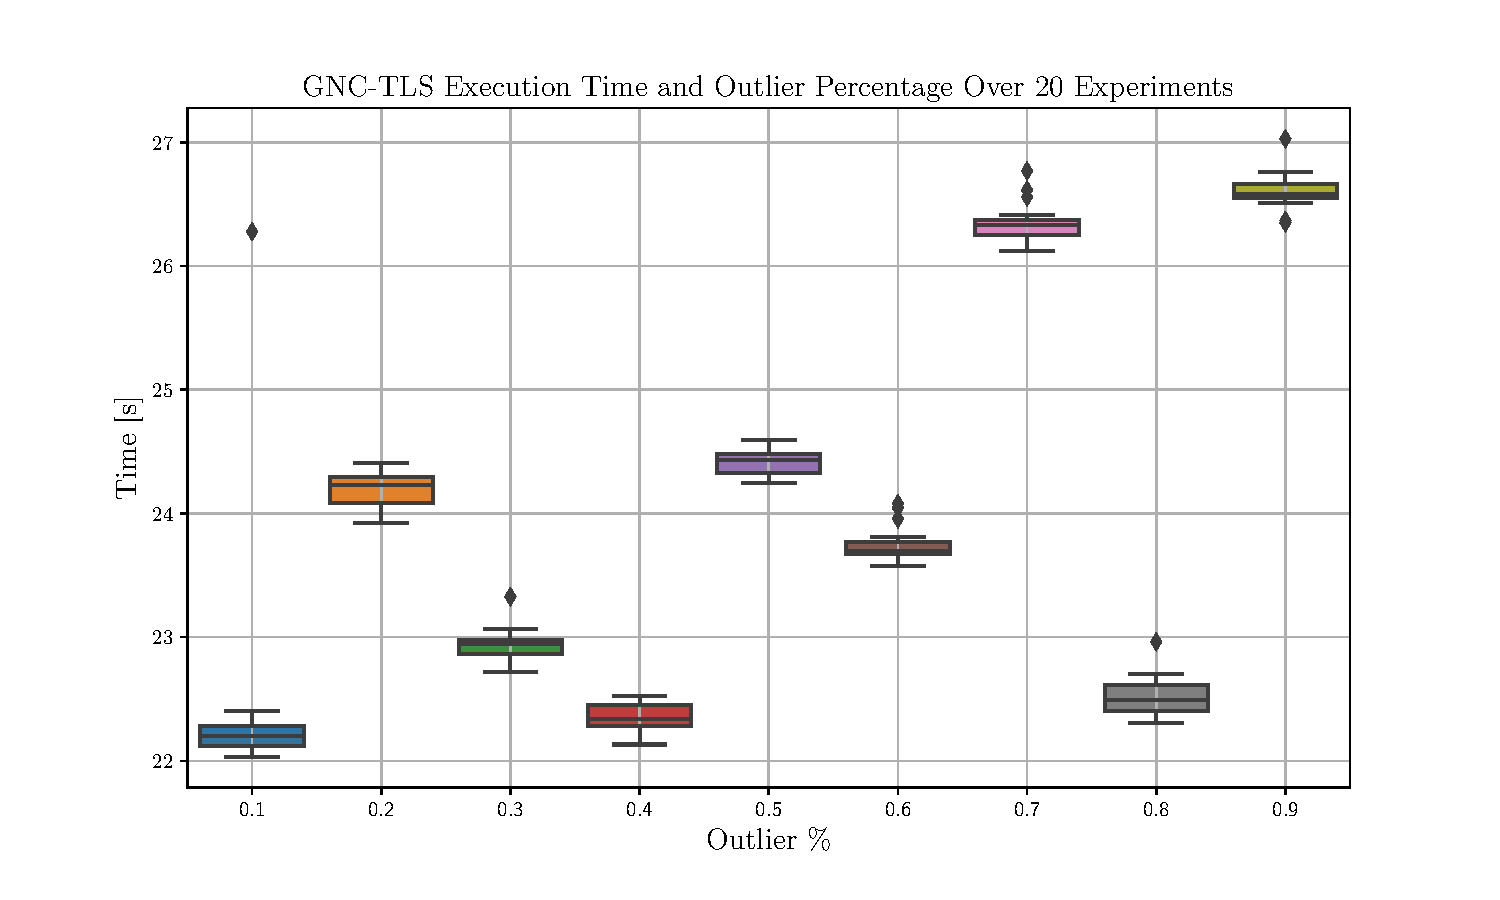
\includegraphics[width=\textwidth]{chapters/2-pose-estimation/fig/GNC-TLS-time-e.pdf}
	\end{center}
	\caption{Boxplots showing the execution time of \gls{gnc} for each outlier percentage from \SI{10}{\percent} to \SI{90}{\percent} in steps of \SI{10}{\percent}, over \num{20} experiments.}
	\label{fig:GNC-TLS-time-e}
\end{figure}

\begin{figure}[!h]
	\begin{center}
		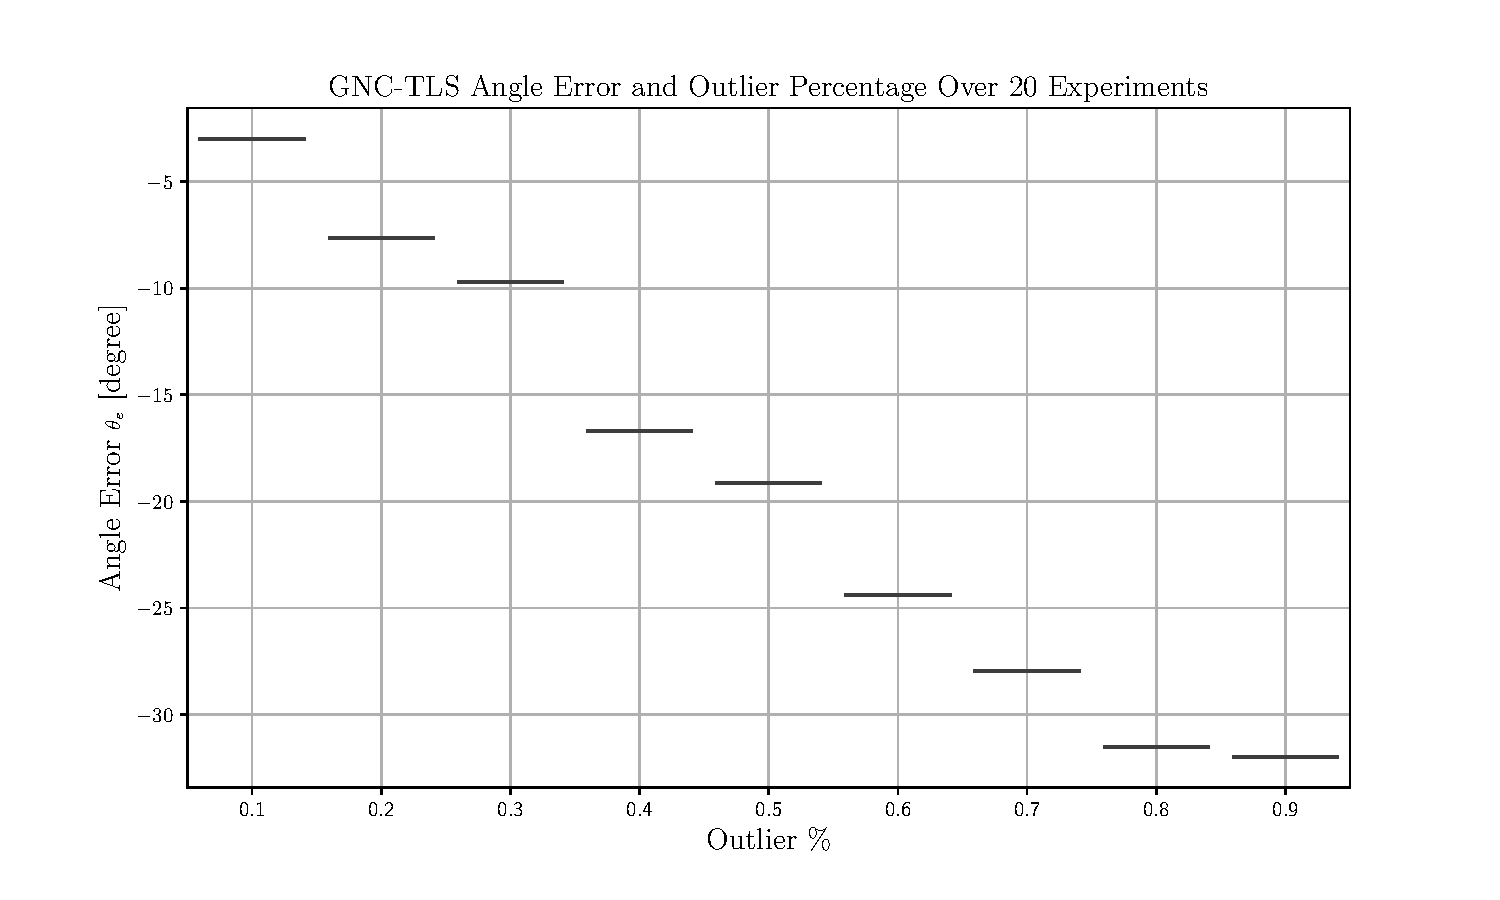
\includegraphics[width=\textwidth]{chapters/2-pose-estimation/fig/GNC-TLS-theta-e.pdf}
	\end{center}
	\caption{Boxplots showing the orientation angle error \mvar{\theta_e} of \gls{gnc}+\gls{rcqp} for each outlier percentage from \SI{10}{\percent} to \SI{90}{\percent} in steps of \SI{10}{\percent}, over \num{20} experiments.}
	\label{fig:GNC-TLS-theta-e}
\end{figure}

\begin{figure}[!h]
	\begin{center}
		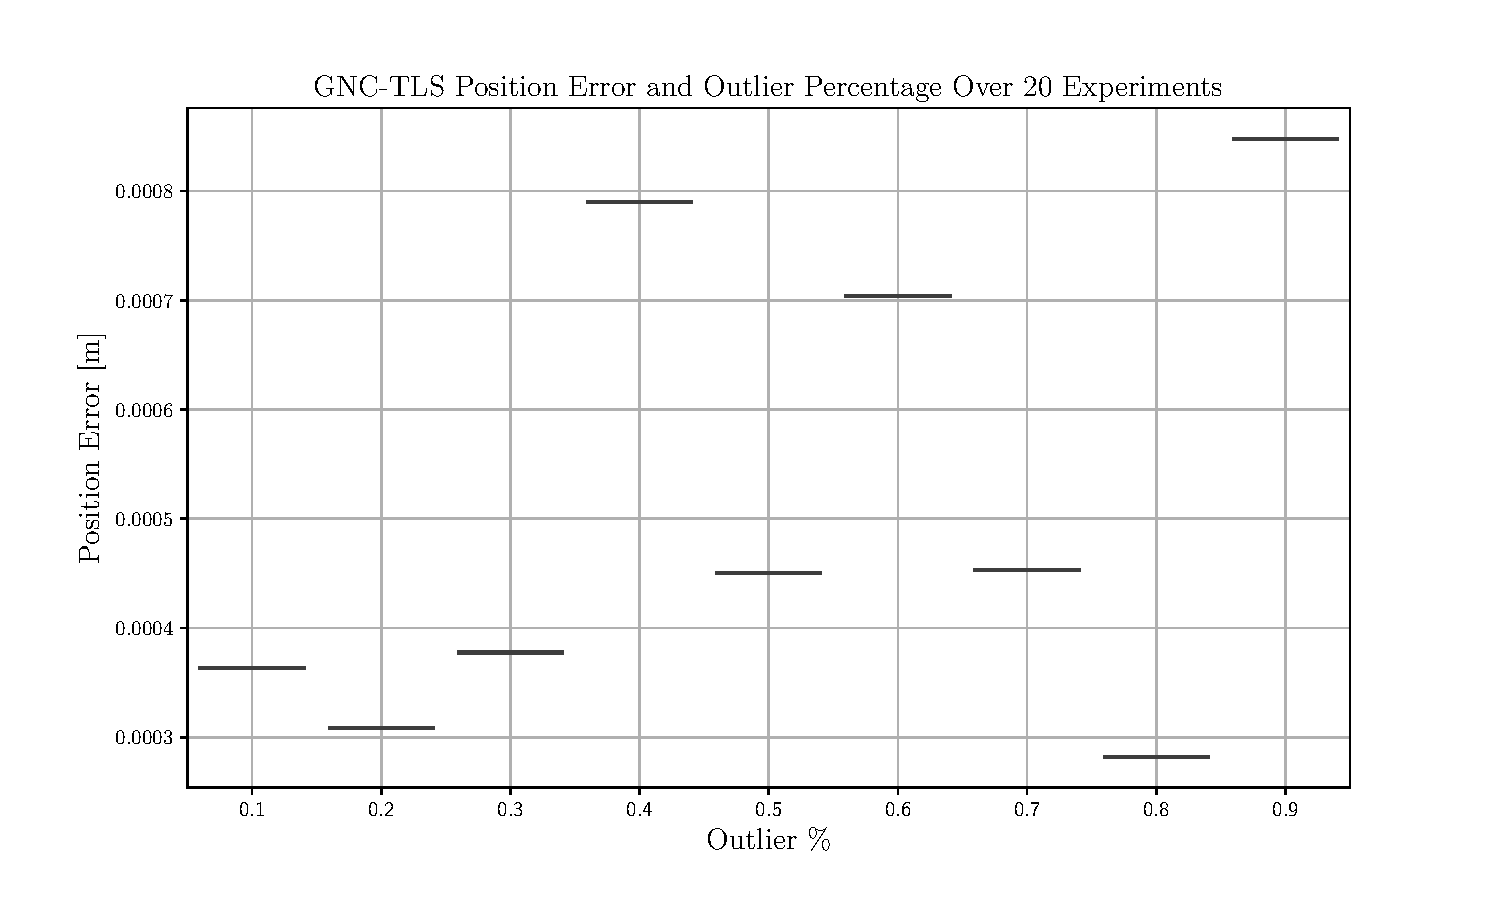
\includegraphics[width=\textwidth]{chapters/2-pose-estimation/fig/GNC-TLS-t-e.pdf}
	\end{center}
	\caption{Boxplots showing the positional error of \gls{gnc}+\gls{rcqp} for each outlier percentage from \SI{10}{\percent} to \SI{90}{\percent} in steps of \SI{10}{\percent}, over \num{20} experiments.}
	\label{fig:GNC-TLS-t-e}
\end{figure}

\newpage
\subsection{Weight Convergence Data}\label{sec:weight-convergence-data}

In~\figref{fig:GNC-TLS-w-history-conv} the weight history is shown for a single run with \SI{10}{\percent} outliers. Here each graph shows a weight entry and how it changes throughout the outer loop iterations. It can here be seen that the weights start at zero and converge either to \num{0} or \num{1} as one would come to expect.\medskip

\figref{fig:GNC-TLS-w-run-conv} show the number of non-zero entries for \num{20} experiments with \SI{10}{\percent} outliers.

\begin{figure}[!h]
	\begin{center}
		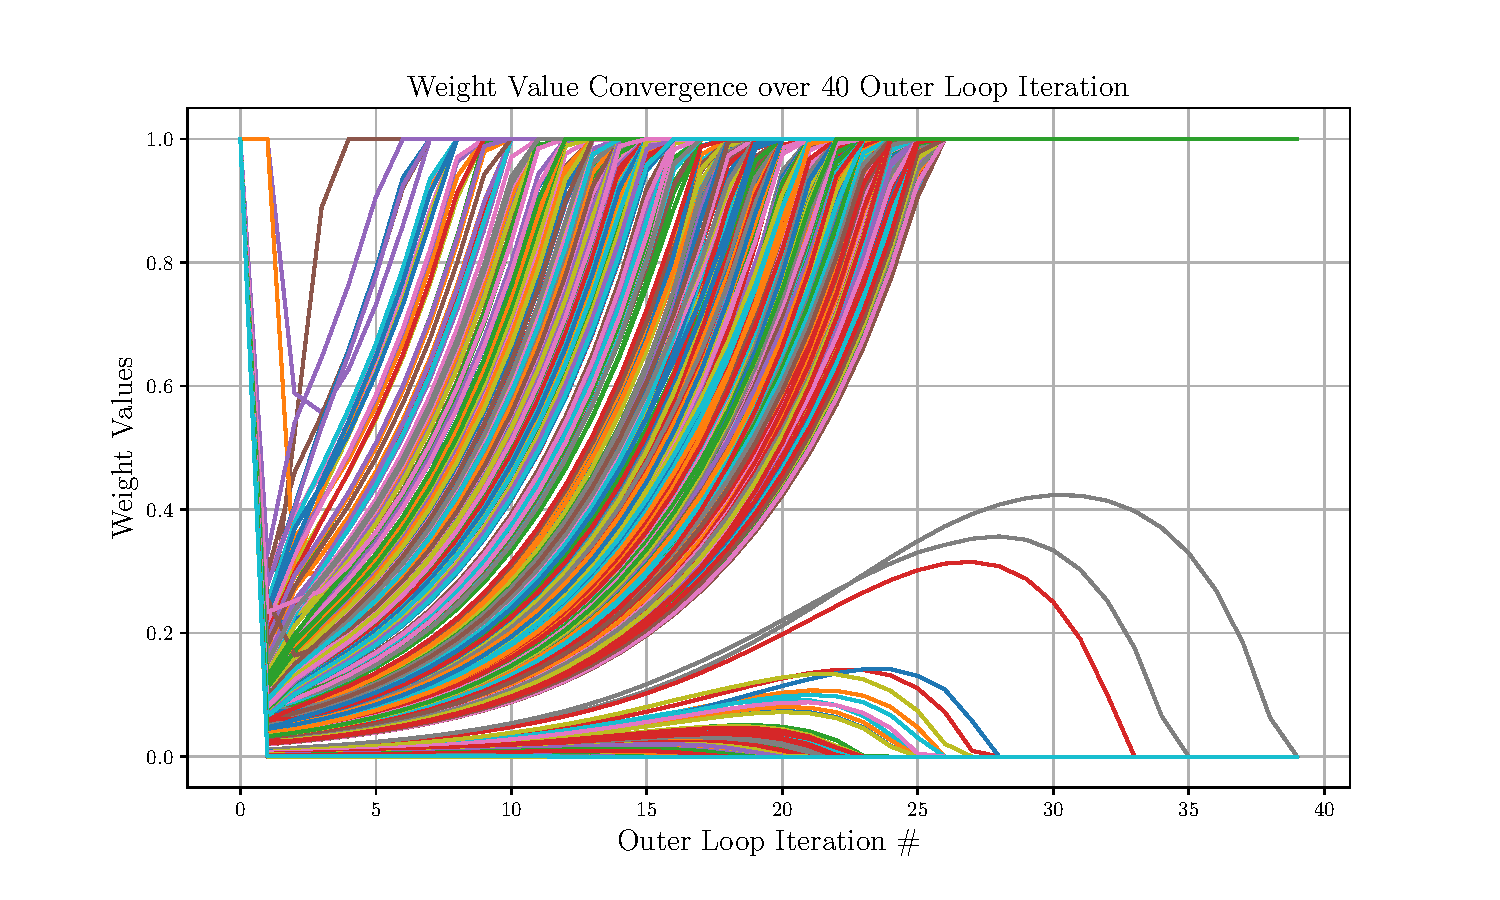
\includegraphics[width=\textwidth]{chapters/2-pose-estimation/fig/GNC-TLS-w-history-conv.pdf}
	\end{center}
	\caption{Weight changes as outer loop iterations pass. This is performed with \SI{10}{\percent} outliers.}
	\label{fig:GNC-TLS-w-history-conv}
\end{figure}

\begin{figure}[!h]
	\begin{center}
		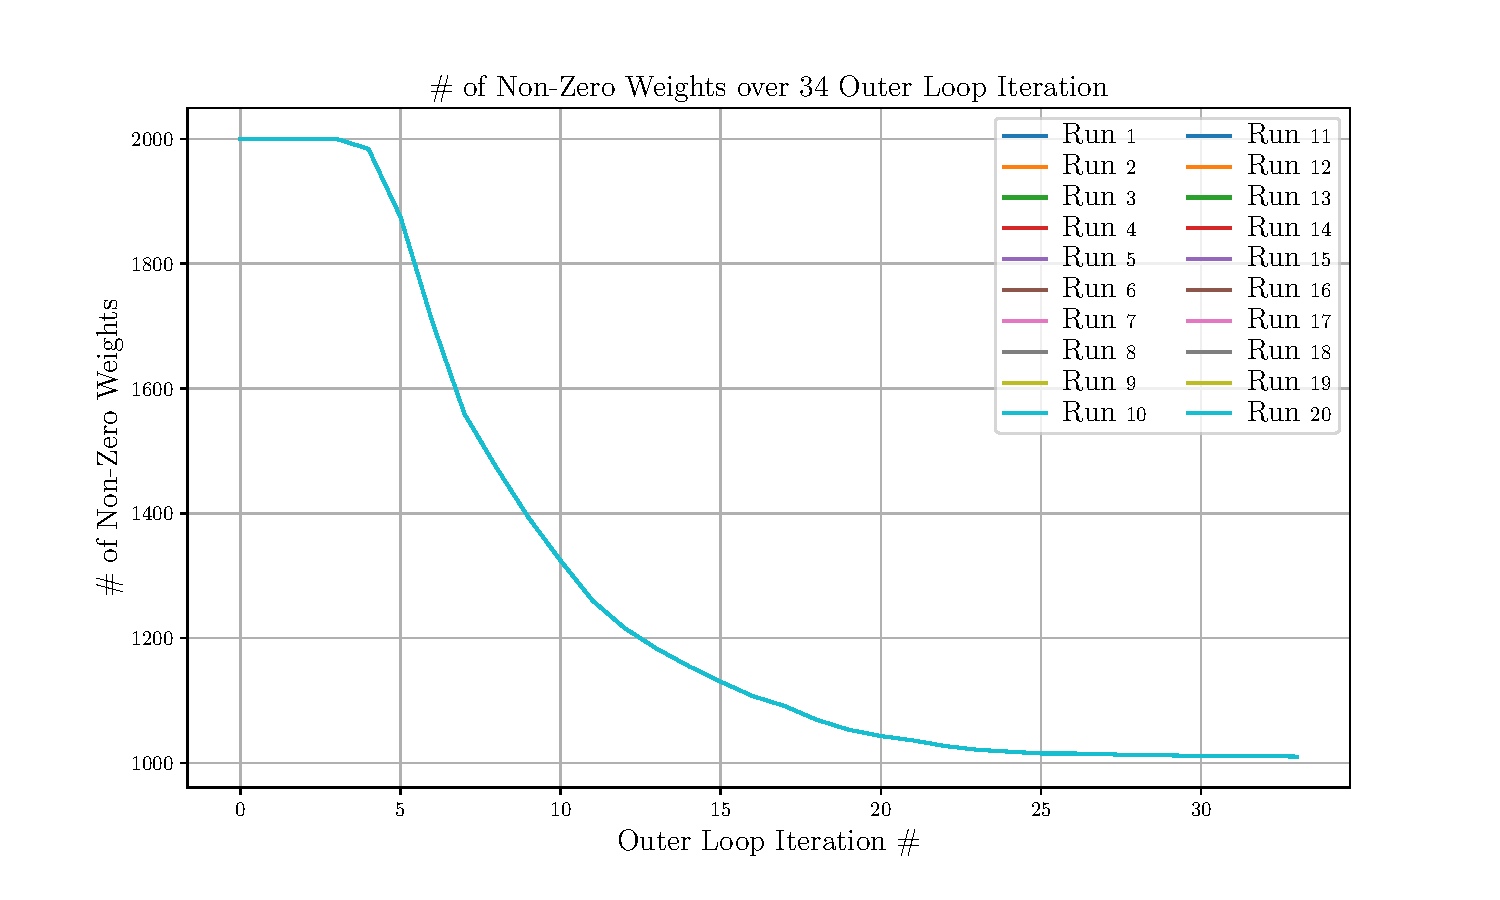
\includegraphics[width=\textwidth]{chapters/2-pose-estimation/fig/GNC-TLS-w-run-10-conv.pdf}
	\end{center}
	\caption{Number of non-zero elements in \vec{\omega} over \num{34} outer loop iterations.}
	\label{fig:GNC-TLS-w-run-conv}
\end{figure}

\section{Discussion \& Conclusion}\label{sec:2-pose-estimation-discussion}

% Given the results from \chapref{ch:1-tactile-perception} to solve problem~\ref{prob:1}, the goal of this chapter is to perform \gls{pe} on a known object.

In this chapter, the pose of the known object, the Stanford bunny, has successfully been estimated from synthetic source data. \medskip

% This chapter focuses specifically on addressing the optimization-based \gls{pcr} problem. It introduces the \gls{rcqp} and \gls{gnc} methods used to solve this problem and evaluates their performance in estimating the pose of the object of interest. The primary objective is to assess the extent to which \gls{rcqp} and \gls{gnc} can accurately estimate the position and orientation of the object, aiming for an orientational error less than \SI{5}{\degree} and a positional error less than \SI{1}{cm}. Importantly, it is assumed throughout the chapter that the object of interest is known, eliminating the need for classification.\medskip

The problem of interest was successfully formalized for two cases, one considering synthetic and one considering sampled source data. Following this, both of the core methodologies \gls{gnc} and \gls{rcqp} were presented, along with the experimental setups for testing both cases. It was found that the sampled source data generated from~\chapref{ch:1-tactile-perception} was insufficient to estimate the object's pose, while the synthetic source data successfully did so. The performance of which fulfilled the presented success criteria of absolute angle errors less than \SI{5}{\degree} and positional errors less than \SI{1}{cm}. This was achieved with an outlier ratio of \SI{10}{\percent} as \mvar{\theta_e\approx -3^\circ} while the positional error, independent of the outlier ratio never exceeded \mvar{\approx} \SI{0.08}{\centi\meter}. However, as the outlier percentage increased to \SI{20}{\percent}, the angle error reached \SI{-7.66}{\degree}, failing to meet the desired success criteria. This trend persisted for higher outlier ratios as well. \medskip

% With outlier ratios greater than \SI{10}{\percent}, the angle error reached \SI{-7.66}{\degree}.
% In the case of synthetic data, the pose estimation problem was successfully solved with satisfactory results for orientation estimation, even in the presence of a \SI{10}{\percent} outlier percentage. However, as the outlier percentage increased to \SI{20}{\percent}, the angle error reached \SI{-7.66}{\degree}, failing to meet the desired success criteria. This trend persisted for higher outlier ratios as well. \medskip
% To achieve this goal, the chapter presents the methodologies employed, the experimental setup, and the obtained results. The results obtained in this chapter are two fold 1) synthetic source data is generated from the target data to ensure \gls{gt} correspondences. This allows for the evaluation of the methods' robustness by introducing varying percentages of outliers. 2) the methods are applied on sampled source data from~\chapref{ch:1-tactile-perception} to estimate the pose of the object based on computed correspondences. The additional challenge in 2) is thus to also solve the \gls{corr-problem} to a degree where the number of feature correspondences allows the algorithms to run. \medskip
% Furthermore, in addition to solving the pose estimation problem, the chapter includes an analysis of the weight involved in \gls{gnc}. Specifically the estimation of the signal-to-outlier ratio and weight convergence. If possible this is performed on both the synthetic and sampled sensor data. \medskip
% Finally, the performance of the presented methods is concluded upon and the extent to which the results are satisfactory is addressed.
The obtained results demonstrate the effectiveness of the \gls{gnc}+\gls{rcqp} method for pose estimation when applied to synthetic data. However, when dealing with sampled data, the methods faced challenges due to the lack of discernible features. One of the main difficulties encountered was the inability to identify a sufficient number of feature correspondences. This limitation can be attributed to the sparsity of the point cloud, indicating the need for intelligent probing techniques to enhance feature detection. \medskip

The execution times and number of iterations appeared consistent with trends demonstrated in the original paper~\cite{graduated-non-convexity-for-robust-spatial-perception:-from-non-minimal-solvers-to-global-outlier-rejection}. \medskip

% In the case of synthetic data, the pose estimation problem was successfully solved with satisfactory results for orientation estimation, even in the presence of a \SI{10}{\percent} outlier percentage. However, as the outlier percentage increased to \SI{20}{\percent}, the angle error reached \SI{-7.66}{\degree}, failing to meet the desired success criteria. This trend persisted for higher outlier ratios as well. \medskip

The weight convergence analysis revealed an expected trend of convergence towards \num{0} and \num{1}. However, the specific values at which the weights converged require further investigation and explanation. For example, in the case of a \SI{10}{\percent} outlier scenario, the expected outcome would be the convergence of the number of non-zero weights to \num{900}, from which an outlier ratio could be computed. Detailed graphs illustrating the weight convergence results can be found in~\appref{app:pose-estimation-weight-convergence}.\medskip

In summary, the \gls{gnc}+\gls{rcqp} method exhibited promising performance in pose estimation for synthetic data. However, challenges arose when working with sampled data, emphasizing the need for improved feature detection and data sampling techniques. The angle error increased with higher outlier percentages, suggesting the importance of robustness in handling outliers. Further analysis is required to understand the convergence values of the weights and refine the pose estimation algorithm accordingly.